% ---------- Präambel ----------

% Schriftgrösse 11, A4 Format, für Artikel, Essays
\documentclass[11pt,a4paper,]{scrartcl}

% Seitenränder einstellen
\usepackage[left=2.5cm,right=2.5cm,top=2.5cm,bottom=2.5cm]{geometry}

% Direkte Angabe von Umlauten im Dokument
\usepackage[utf8]{inputenc}

% Deutsche Sprachanpassungen
\usepackage[ngerman]{babel}

% Schriftart im gesamten Dokument einstellen
%\usepackage{kpfonts}
\renewcommand*{\familydefault}{\sfdefault}

% Silbentrennung bei Sonderzeichen
\usepackage[T1]{fontenc}

% Mathematische Formeln aktivieren
\usepackage{amsmath}

% Schriftarten in Mathematischen Formeln
\usepackage{amsfonts}

% Bildpositionen erzwingen
\usepackage{float}

% Mathematische Symbole aktivieren
\usepackage{amssymb}

% Textboxen aktivieren
\usepackage{framed}

% Glossar
\usepackage[acronym, automake]{glossaries}
\makeglossaries
% Remove Title from Glossaries
\renewcommand{\glossarysection}[2][]{}
\setlength{\glsdescwidth}{0.8\textwidth}

%PDF einfügen
\usepackage{pdfpages}

% Zitationsstil
%\usepackage{cite}
%\bibliographystyle{ieeetr}
\usepackage[backend=biber, defernumbers=true, style=ieee]{biblatex}
\addbibresource{Verzeichnisse/Literatur.bib}
\usepackage{url}
\assignrefcontextkeyws[labelprefix=L]{L}
\assignrefcontextkeyws[labelprefix=Q]{Q}

% Grafiken einbinden
\usepackage{graphicx}
\usepackage{subfigure}
\newcommand{\fref}[1]{\figurename\ \ref{#1}}

% Tabellen rotieren
\usepackage{rotating}
\usepackage{adjustbox}
\newcommand{\tref}[1]{\tablename\ \ref{#1}}

% Autor setzen
\author{\TheAuthor}

% Titel setzen
\title{\TheTitle}

% Inhaltsverzeichnis Stil
\usepackage{tocstyle}
\newtocstyle[KOMAlike][leaders]{alldotted}{}
\usetocstyle{alldotted}
 

% -------- Variabeln --------
% Autor
\newcommand{\TheAuthor}{Josef Böckle \& Daniel Lüchinger}
\newcommand{\TheAuthorShort}{Böckle, Lüchinger}
% Titel
\newcommand{\TheTitle}{Fast and Curious\\ \begin{Large}
Dokumentation
\end{Large}}
% Projektname
\newcommand{\projektName}{Fast and Curious}
% Auftraggeber
\newcommand{\auftraggeber}{Adlos AG, Thomas Vogt}
% Referent
\newcommand{\RefName}{Klaus Frick}
 % Koreferent
\newcommand{\coRefName}{Tindaro Pittorino}

% ---------- Kopfzeile & Fusszeile ----------
% Kopf und Fusszeile aktivieren
\usepackage{fancyhdr}
% Keine vorgefertigte Kopf/Fusszeilen verwenden
\pagestyle{fancy}
% Eigentliche Kopfzeilen Einstellung
\lhead{Fast and Curious}
\chead{}
\rhead[]{\nouppercase{\leftmark}}
\lfoot{\TheAuthorShort}
\cfoot{\jobname .pdf}
\rfoot{Seite \thepage}
% Linien
\renewcommand{\footrulewidth}{0.4pt} %untere Trennlinie
\renewcommand{\headrulewidth}{0.4pt} %untere Trennlinie

% Aufzählungsart
\usepackage{enumitem}
\newlist{citemize}{itemize}{4}
\setlist[citemize]{label=\textbullet,nosep,topsep=-\parskip}

% ---------- Eigentliches Dokument ----------
\begin{document}
\begin{titlepage}
	
\includegraphics[height=0.05\textheight]{Deckblatt/NTB.jpg}
	\hfill
  	
\includegraphics[height=0.05\textheight]{Deckblatt/ICE.jpg}
  	
	\thispagestyle{empty} % no page number
	
	\vspace{6cm}
	
	\centering
	
	
	\begin{huge} 
		Bachelorarbeit
	\end{huge}
	
	\vspace{2cm}

	\fontsize{45pt}{30pt}\selectfont
	\textbf{Fast and Curious }

	

	\vspace{1cm}
	
	\fontsize{20pt}{20pt}\selectfont	
	Entwicklung eines Low-Cost Verkehrsflussmesssystems 
	\fontsize{11pt}{11pt}\selectfont	

\begin{verbatim}











\end{verbatim}

\begin{center}
  \begin{tabular}[p{3cm}p{10cm}p{3cm}]{ccc}
  \\
	Josef Böckle      & & Daniel Lüchinger \\[1.2ex]
	Brauentinweg 12  & & Oberauweg 5d \\[1.2ex]
	6713 Ludesch 	   & & 9453 Eichberg \\ [1.2ex]
	josef.boeckle@ntb.ch   & & daniel.luechinger@ntb.ch\\\\\\ [1.2ex]
	& \large{\today} &
  \end{tabular}

\begin{verbatim}


\end{verbatim}


\includegraphics[height=0.05\textheight]{Deckblatt/Adlos.jpg}
\end{center}
\end{titlepage}

\setcounter{page}{1} 
\setlength{\parindent}{0em}
\setlength\tabcolsep{0pt}
\tableofcontents
\newpage 
\section{Danksagung}
\newpage

\section{Abstract}
Das Ziel von Fast and Curious war es, ein System zu entwickeln, welches als einzelnes Gerät vorbeifahrende Verkehrsteilnehmer zählt, kategorisiert und eine grobe Aussage über dessen Geschwindigkeit aussagen kann. Als System von Geräten sollte es zudem eine statistische Aussage über das Fahrverhalten der aufgezeichneten Verkehrsteilnehmer treffen können. Ebenfalls mussten die Rahmenbedingungen von tiefen Kosten und einer langen Laufzeit eingehalten werden. Das gesamte System sollte bei jeder Witterung einsatzfähig sein und am Strassenrand einer maximal zweispurigen Strasse platziert werden. Das Gerät sollte an einer Strassenlaterne auf einer Höhe von sechs Meter befestigt werden.\\\\
Ein einzelnes Gerät besteht aus einer Rechnereinheit mit einem Quad-core Prozessor, welcher in der Lage ist, mehrere Prozesse parallel abzuarbeiten. Dies ist notwendig um eine beinahe Echtzeitauswertung gewährleisten zu können. Um die Verkehrsteilnehmer einzeln zu identifizieren, wird eine Kamera mit hoher Bildrate, jedoch geringer Auflösung verwendet. Um eine Messung an jeder beliebigen Strassenlaterne durchführen zu können, wird eine externe Stromversorgung benötigt, welche das Gerät über mehrere Tage hinweg einsatzfähig macht. Damit sich die Geräte in der richtigen Position befinden, wird mithilfe eines WIFI-Adapters eine Verbindung zu einem Endgerät herstellt. Dabei muss vom Benutzer ein Hotspot errichtet werden, auf welchen sich das Gerät verbindet. Mithilfe einer Website kann im Anschluss das Gerät gesteuert und überwacht werden. Um das Gerät parallel zur Strasse ausrichten zu können, wird auf der Website ein Live-Stream der Kameraposition angezeigt. Dadurch kann die genaue Ausrichtung justiert und das Gerät im Anschluss gestartet werden.\\\\
Im Betriebsmodus beschäftigt sich der erste Kern permanent mit der Aufnahme von Videos, welche nach 15 Minuten abgespeichert werden. Ein weiterer Kern analysiert die aufgenommenen Videos, indem jeweils zwei aufeinanderfolgende Frames verglichen werden. Somit können Bewegungen erkannt und Bilder mit Bewegungen temporär gespeichert werden. Nachdem das Video abgearbeitet wurde, wird es vom temporären Speicher entfernt. Der dritte Kern verwendet die Bilder, auf welchen Bewegungen erkannt wurden und verknüpft diese logisch miteinander um einen Verkehrsteilnehmer identifizieren zu können. Daraus werden zu jedem Verkehrsteilnehmer Eigenschaften extrahiert und in einem Feature Vektor gespeichert. Zu den extrahierten Eigenschaften gehört ein Zeitstempel, die Fahrtrichtung, ein Zähler für die Anzahl Fahrzeuge pro Fahrtrichtung, eine Kategorisierung sowie eine Geschwindigkeitseinteilung. Dieser Feature Vektor wird später verwendet, um den Verkehrsfluss in einem begrenzten Gebiet rekonstruieren und daraus eine statistische Aussage treffen zu können. Der letzte Kern beschäftigt sich mit der Steuerung und Überwachung der anderen Kerne. Dies ist notwendig, um garantieren zu können, dass den Prozessen jederzeit genügend Ressourcen zur Verfügung stehen. Und ausserdem, um kleinere Aufgaben nebenbei durchführen zu können. Dies beinhaltet das Monitoring der Rechnereinheit sowie das Handeln des Webservers, damit auf Eingaben des Benutzers reagiert werden kann.\\\\
Nachdem das Gerät entwickelt und ersten Tests standgehalten hatte, wurde ein erster Feldversuch mit mehreren Geräten in der Gemeinde Satteins im Vorarlberg durchgeführt. Dabei wurden sechs Geräte zur selben Zeit an verkehrsrelevanten Stellen angebracht und über eine Dauer von mehreren Tagen in Betrieb gehalten. Aus den gewonnenen Daten wurde zum einen die Anzahl Verkehrsteilnehmer an jedem Gerät gezählt und kategorisiert, zum anderen wurde der Verkehrsfluss in der Gemeinde Satteins statistisch rekonstruiert und dargestellt. Anhand von Testbildern, welche gleichzeitig aufgenommen wurden, konnte eine hohe Übereinstimmung des Verkehrsflusses nachgestellt werden.\\\\
In weiteren Arbeiten könnten die Geräte eine Echtzeitauswertung realisieren, welche jederzeit online abrufbar wäre. Dazu müssten die Geräte entweder ihre Daten auf einen Online-Server transferieren, oder mittels LoRa-WAN an einen Host übertragen. Ebenfalls wäre es möglich, die Geräte mit zusätzlichen Sensoren zu erweitern, sodass weitere verkehrsrelevante Daten wie Lautstärkemessungen, Wettersituation oder Schadstoffmessungen aufgenommen werden.
\newpage
\section{Einleitung}
\subsection{Aufgabenstellung}
Die Aufgabe dieses Projektes war es, ein Gerät zu entwickeln, welches autonom vorbeifahrende Verkehrsteilnehmer erkennt und im Anschluss diverse Operationen auf diese ausführt, um somit eine genaue Identifikation dieser Verkehrsteilnehmer zu erreichen. Das Gerät sollte zwei verschiedene Zähler beinhalten, welche sowohl links als auch rechtsfahrende Fahrzeuge unabhängig voneinander zählen kann. Zudem sollte das Gerät die aufgenommenen Fahrzeuge je nach Grösse in verschiedene Kategorien unterteilen und ebenfalls eine grobe Abschätzung über die momentane Geschwindigkeit aussagen können.  Mit zusätzlichem Zeitstempel, welcher bei der Vorbeifahrt der einzelnen Fahrzeuge aufgenommen wurde, sollten alle gefunden Indikatoren in eine Tabelle eingetragen werden, damit diese für spätere Auswertungen verwendet werden kann.  Ein Gerät sollte etwa eine Woche ohne Unterbruch im Betrieb bleiben und zusätzlich die Speicherkarte in dieser besagten Zeit nicht überfüllen. Das einzelne Gerät soll möglichst einfach aufgestellt werden können und dennoch ein gewisses Monitoring möglich sein. Im besten Fall soll eine Ausrichtung mithilfe des Mobilphones durchgeführt werden können und ebenfalls die momentane Ausrichtung ohne grossen Zeitaufwand kontrolliert und korrigiert werden können.\\
Damit eine Verkehrsverfolgung durchgeführt werden kann, sollen die einzelnen Geräte zu einem System gekoppelt werden können. So sollen die Fahrzeuge an mehreren Orten von mehreren Geräten wiedererkannt werden und damit der stattgefundene Verkehrsfluss der Teilnehmer rekonstruiert werden können. Durch strategisch günstige Positionen der Geräte und geeignete Algorithmen sollen nur ein Bruchteil aller aufgenommenen Fahrzeuge für die Wiederidentifikation eines Teilnehmers in Betracht kommen und somit eine genauere und schnellere und Auswertung erreicht werden. Dabei soll es sich um eine statische Aussage handeln, weshalb nicht zwingend jeder Verkehrsteilnehmer exakt erkannt werden muss. Dies wurde so bestimmt, da die Verkehrsteilnehmer "'verschwinden"' können, falls diese im Ort wohnen oder für längere Zeit anderweitig beschäftigt sind.\\
Damit die Verkehrsverfolgung gelingen kann, müssen neben den bereits erwähnten Indikatoren noch weitere Eigenschaften gefunden werden, um die Fahrzeuge genauer einteilen zu können. Was für Indikatoren der Tabelle hinzugefügt werden, sollte sich im Verlauf dieser Bachelorarbeit zeigen. Eine gewisse Auswertung der aufgenommenen Resultate solle ebenfalls visualisiert werden. Bestenfalls könnte dies mithilfe von Open Source Tools wie beispielsweise Open Street Map geschehen.
\input{Einleitung/Wertschöpfung}
\newpage
\section{Fast and Curious}
\subsection{Anforderungen}
\subsubsection{Robustheit}
\subsubsection{Laufzeit}
\subsubsection{Verarbeitungszeit}
\subsubsection{Kosten}
\input{FastAndCurious/Umwelteinflüsse}
\newpage
\section{Hardware}
\subsection{Komponenten}
Bei den Komponenten musste darauf geachtet werden, dass diese den äusseren Einflüssen sowie den spezifischen Softwaretechnischen Daten genügen. Die einzelnen Geräte der Arbeit bestehen aus Rechnereinheit, Messsensor, WIFI-Adapter, Gehäuse sowie einer Spannungsversorgung.

\subsubsection{Rechnereinheit}
An die Rechnereinheit wurden sehr grosse Anforderungen gestellt, da diese bei $-40^\circ\text{C}$ aber auch bei über $40^\circ\text{C}$ die Auswertung korrekt durchführen muss. Ebenso muss die Rechnereinheit sehr viel Auswertungen direkt durchführen, um so wenig wie möglich direkt zu speichern. Der Rechnerkern des Gerätes besteht aus einem Allwinner H3, welcher einen Quad-core Cortex-A7 mit bis zu 1.2 GHz Taktrate besitzt. Dieser Rechnerkern ist einer der am Besten geeignetsten für das Gerät, da auf diesem mehrere Prozesse gleichzeitig ablaufen können. Dies ist nötig um die gewünschte Verarbeitungsgeschwindigkeit zu erreichen. Im Zuge dessen wurde ein vorgefertigtes Board im Gerät eingesetzt. Das eingesetzte Board ist ein NanoPi NEO von FriendlyARM \cite{NanoPi}. Der NanoPi NEO hat den oben genannten Quad-core Prozessor, mitwelchem die Aufgabe gelöst werden kann. \\
Dieses Board bietet ebenso den Vorteil, dass sich alles auf einer Fläche von 40x40 cm  befindet. So kann das gesamte Gerät sehr kompakt gestaltet werden. Das Board wird mit einer externen Speicherkarte verwendet, auf welcher sich das Betriebssystem befindet. Im Falle von Fast and Curious ist es Ubuntu 16.04 (Long Time Supported). \\
Nachteil am NanoPi NEO sind zum einen die eher schlechte Dokumentation sowie das Vorhandensein von lediglich eines einzelnen USB Anschlusses. Aus diesem Grunde musste beim  Gerät ein USB Hub verwendet werden um den Messsensor sowie den USB-WIFI-Adapter anzuschliessen. Nachfolgendes Bild (\fref{bLayout}) zeigt das Layout des NanoPi NEO.

\begin{figure}[H]
  \centering
  \includegraphics[width=0.99\textwidth]{Hardware/NanoPi_Neo.jpg} 
  \caption{Layout des NanoPi NEO. \cite{NanoPiNeo}}
  \label{bLayout}
\end{figure}

\subsubsection{Messsensor}
Der Messsensor des Gerätes muss in der Lage sein, Daten der Verkehrsteilenehmer zu liefern, mit denen dann die weitere Auswertung geschehen kann. Es müssen aus den Daten des Messsensors Kenngrössen extrahiert werden, welche die Verkehrsteilnehmer eindeutig identifizieren lässt. Es wurde auf eine Kamera zurückgegriffen, welche im Stande ist zwei Fahrspuren zu überdecken und mindestens drei Bilder pro vorbeifahrendem Verkehrsteilnehmer aufzunehmen. \\
Mithilfe nachfolgender Berechnung wurde die geeignete Kamera sowie das passende Objektiv dazu gefunden. Die Skizze (\fref{bBerechnung}) zeigt die schematische Darstellung eines Aufstellpunktes des Geräts.
\begin{citemize}

\item Kamera mit 30 FPS \\
$l_{ 1,30 } = \frac{ 22.22 m/s }{ 30 FPS} = 0.75 m$ \\ 
$l_{ 4,30 } = 4 * l_{1,30} = 3 m$\\
$\alpha_{30} = 2* \arctan(l_{4,30 }) \approx 150^\circ$ \\\\


\item Kamera mit 60 FPS \\
$l_{ 1,60 } = \frac{ 22.22 m/s }{ 60 FPS} = 0.37 m$ \\ 
$l_{ 4,60 } = 4 * l_{1,30} \approx 1.5 m$\\
$\alpha_{60} = 2* \arctan(l_{4,60 }) \approx 120^\circ$ \\\\
\end{citemize}

\begin{figure}[H]
  \centering
  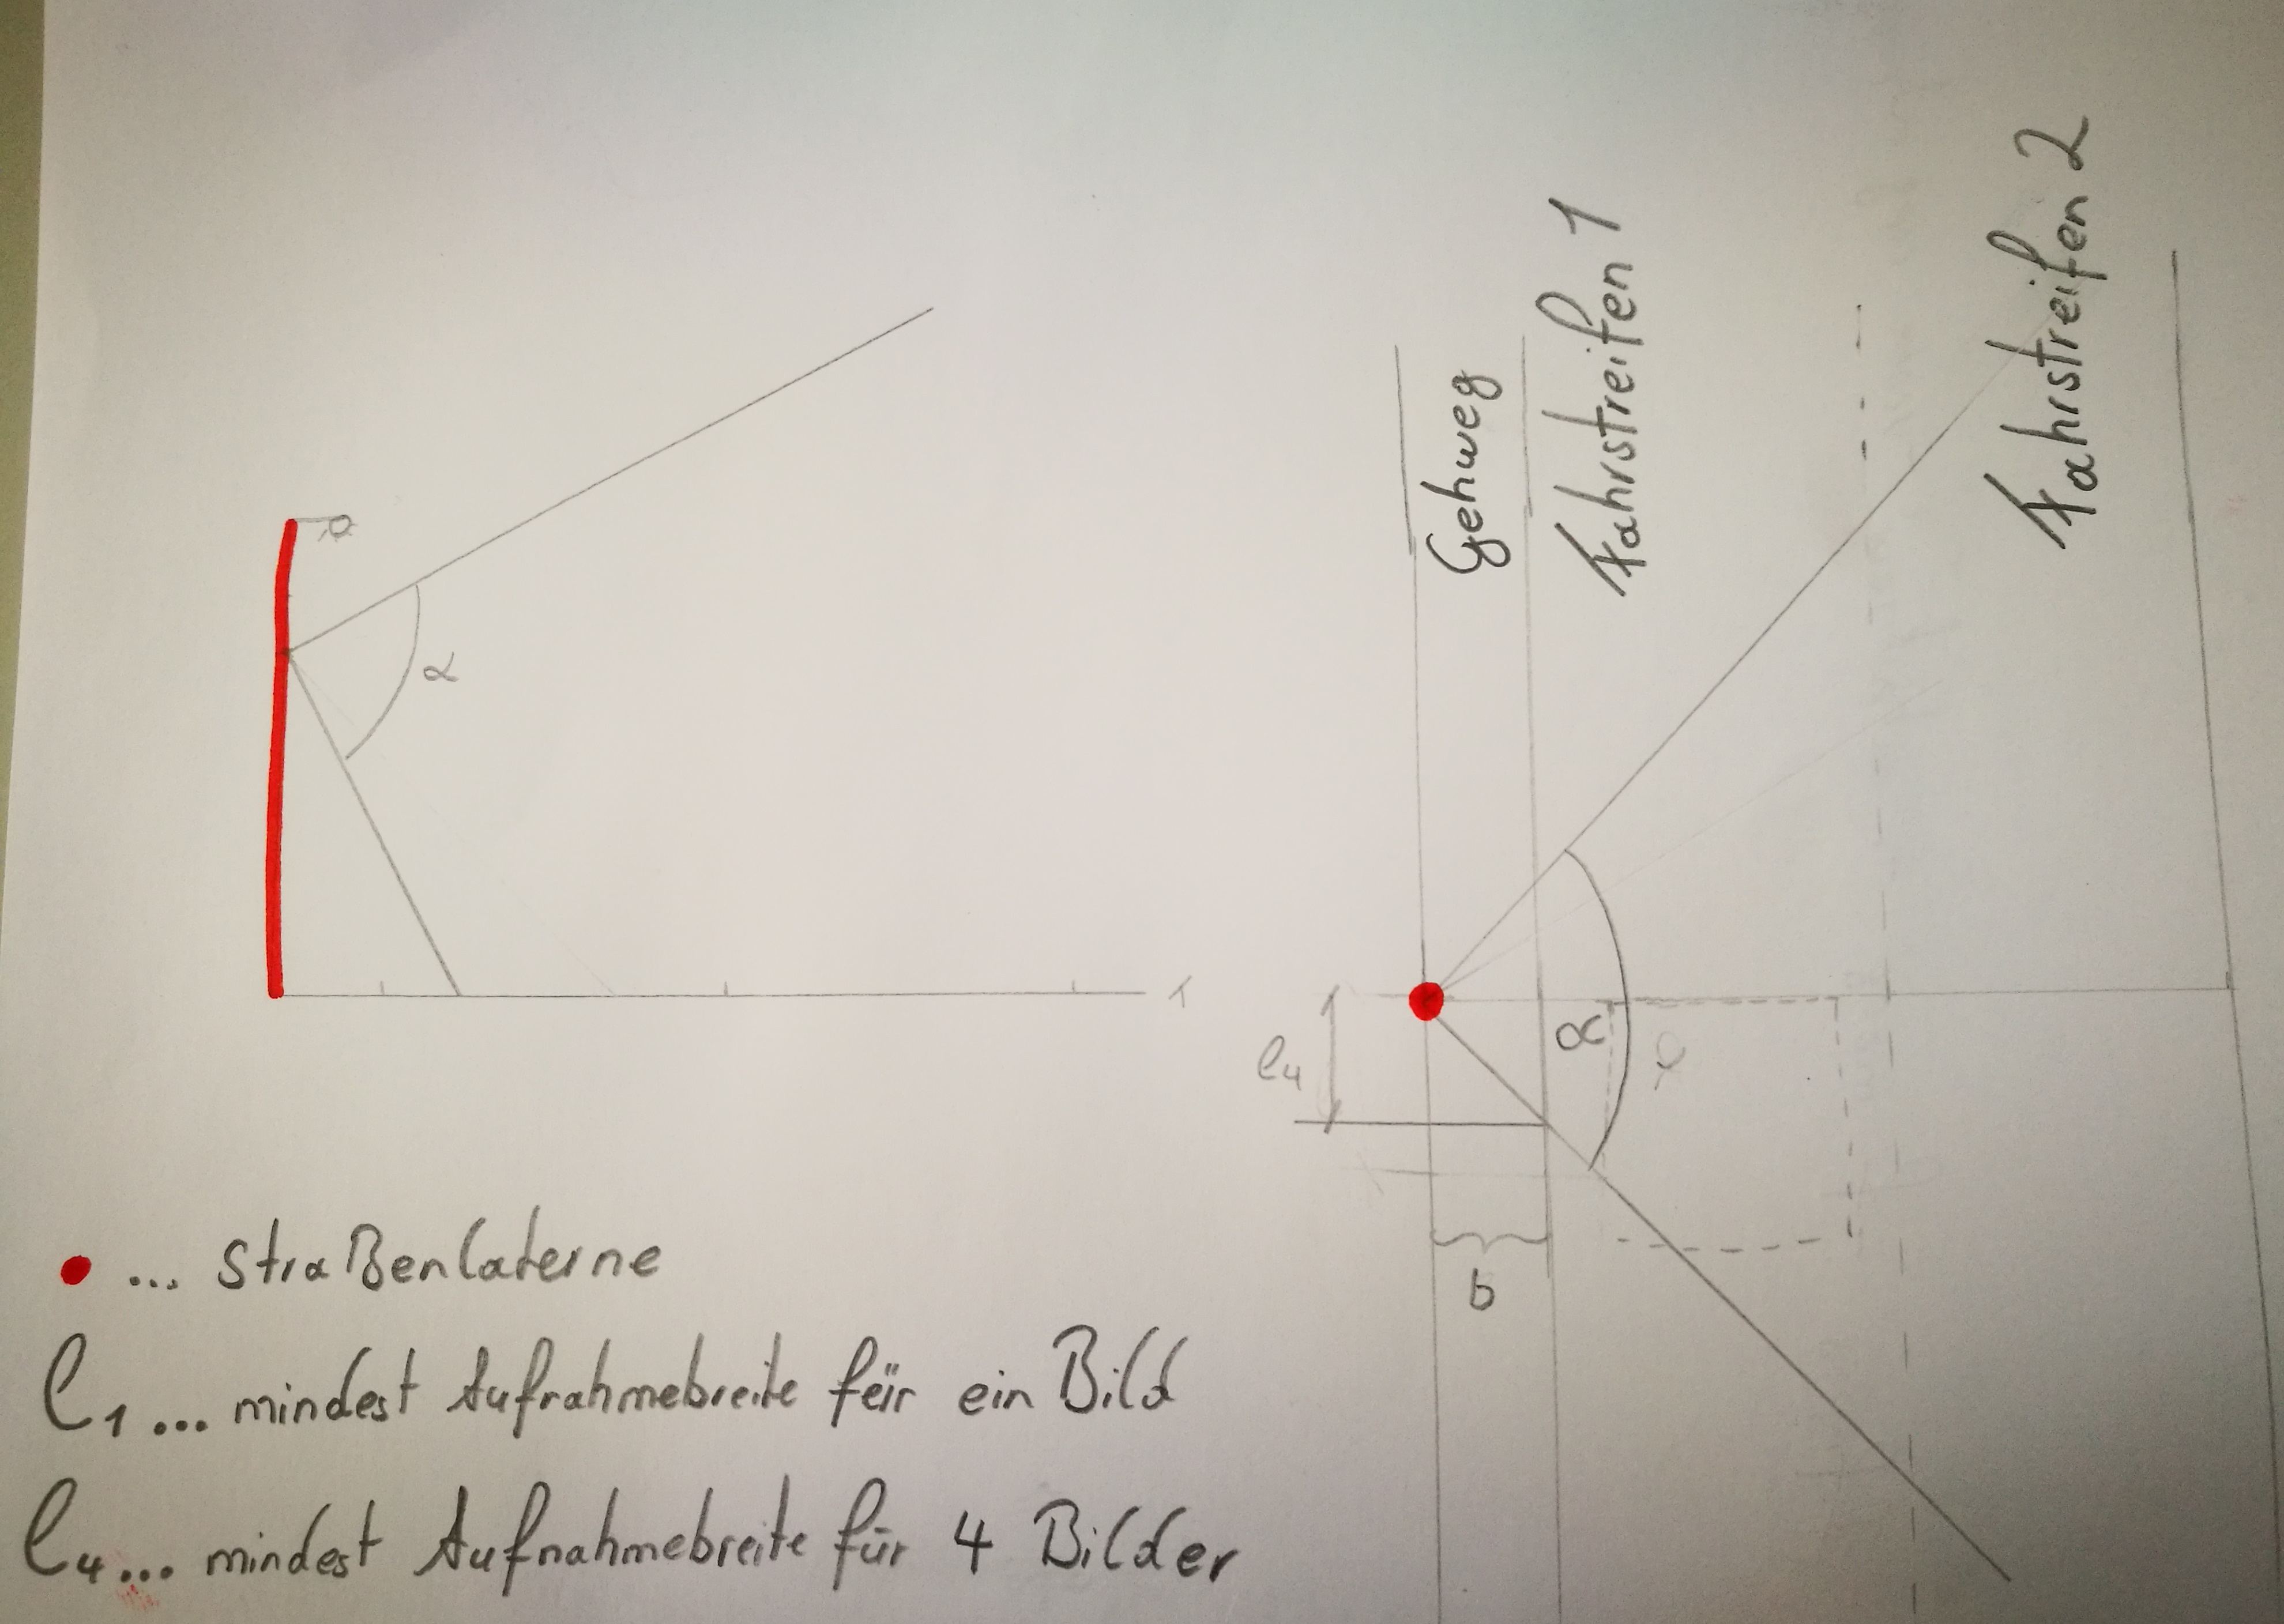
\includegraphics[width=0.99\textwidth]{Hardware/ObjektivBerechnung.jpg} 
  \caption{Skizze zur Berechnung der Kamera Daten.}
  \label{bBerechnung}
\end{figure}

Durch diese Berechnung wurde eine Kamera eingesetzt, welche mit einer Framerate von 60 FPS Bilder aufnimmt. \\
Im produzierten Prototypen wurde eine "'ELP 1080p Full HD H.264"' Kamera mit 3.6 mm Objektiv verwendet. Diese Kamera hat den Vorteil, dass die gewünschten Treiber auf dem Betriebssystem schon installiert sind und die Kamera sehr preisgünstig zu haben ist. Diese Kamera besitzt bei einer FPS Anzahl von 60 eine Auflösung von 640x480 Pixel und einem 3.6 mm Objektiv. Diese Anzahl an Pixel reicht aus, um die nötigen Daten der Verkehrsteilnehmer zu extrahieren. \cite{Kamera}

\subsubsection{WIFI-Adapter}
Um das Gerät Steuern und Überwachen zu können, wird eine kabellose Verbindung benötigt. Dies ist am einfachsten über eine WIFI-Verbindung zu erreichen. Da das NanoPi NEO keine internen Funksender eingebaut hat, wird ein WIFI-Adapter benötigt. Dazu kann jeder WIFI-Adapter verwendet werden, welche das Linux System unterstützen und somit ein Treiber vorhanden ist. Werden für die Geräte unterschiedliche WIFI-Adapter eingesetzt, so muss nach der Anleitung für die Installation der Geräte vorgegangen werden und die Namen der Adapter geändert werden.\\
Die einzige Anforderung an den WIFI-Adapter ist es, dass dieser über USB angeschlossen wird. Die Geräte, welche produziert wurden, haben unterschiedliche WIFI-Adapter eingebaut und es funktioniert mit allen WIFI-Adaptern ohne irgendwelche Probleme. Die Verbindung geschieht über einen Hotspot vom Endgerät zu NanoPi NEO.

\subsubsection{Spannungsversorgung}
Die Spannungsversorgung der Geräte wurde mittels Autobatterie und Spannungswandler realisiert. Das gesamte Gerät benötigt bei Volllast ca. 400 mA Strom. Die verwendeten Autobatterien haben eine Kapazität von 44 Ah und eine Spannung von 12 V. \\

$\frac { 44000\quad mAh\quad \times \quad 12\quad V }{ 400\quad mAh\quad \times \quad 5\quad V } =\quad 264\quad h=\quad 11 d$ \\

Wie aus dieser Berechnung entnommen werden kann, beläuft sich die Betriebszeit mit einer Akku Ladung theoretisch auf ca. 11 Tage. Wie erwartet ist die tatsächliche Laufzeit der Geräte kleiner als die Berechnete. Jedoch beträgt die tatsächliche Laufzeit etwa die Hälfte von ca. 5 Tagen. \\
In einer tatsächlichen Fertigung der Geräte muss eine neue Spannungsquelle gefunden werden, da Autobatterien beinahe immer Bleihaltig sind. Es könnten Lithium Ionen Akkus verwendet werden, jedoch waren diese für die Prototypen zu teuer und nicht rentabel. 

\subsubsection{Gehäuse}
Das Gehäuse der Prototypen besteht aus einer Kunststoffbox, in welcher sich früher Lebensmittel befanden. In diesem Gehäuse wurden alle Komponenten welche oben genannt wurden, mittels Klettverschluss angebracht, um die Komponenten ohne Gehäuse weiter zu verwenden. Dies ermöglichte eine leichtere Bedienung bei der Programmierung der Software. Am Gehäuse wurden zwei Gewindestangen angebracht, um die Ausrichtung des Gerätes einstellen zu können. Des Weiteren wurde im Deckel der Kunststoffboxen Schlitze geschnitten, um die Abwärme der Komponenten besser nach aussen zu befördern. Die Gehäuse werden an den Strassenlaternen mittels grossen Kabelbindern befestigt.\\
\textbf{Wichtig: In den Gehäusen befindet sich keine Batterie.}\\
Aus Sicherheitsgründen wurde ein zweipoliges Kabel von den Geräten nach unten gezogen und an den Polen der Batterie befestigt. Das folgende Bild (\fref{bGehäuse}) dient dabei zur Illustration des leeren Gehäuses.

\begin{figure}[H]
  \centering
  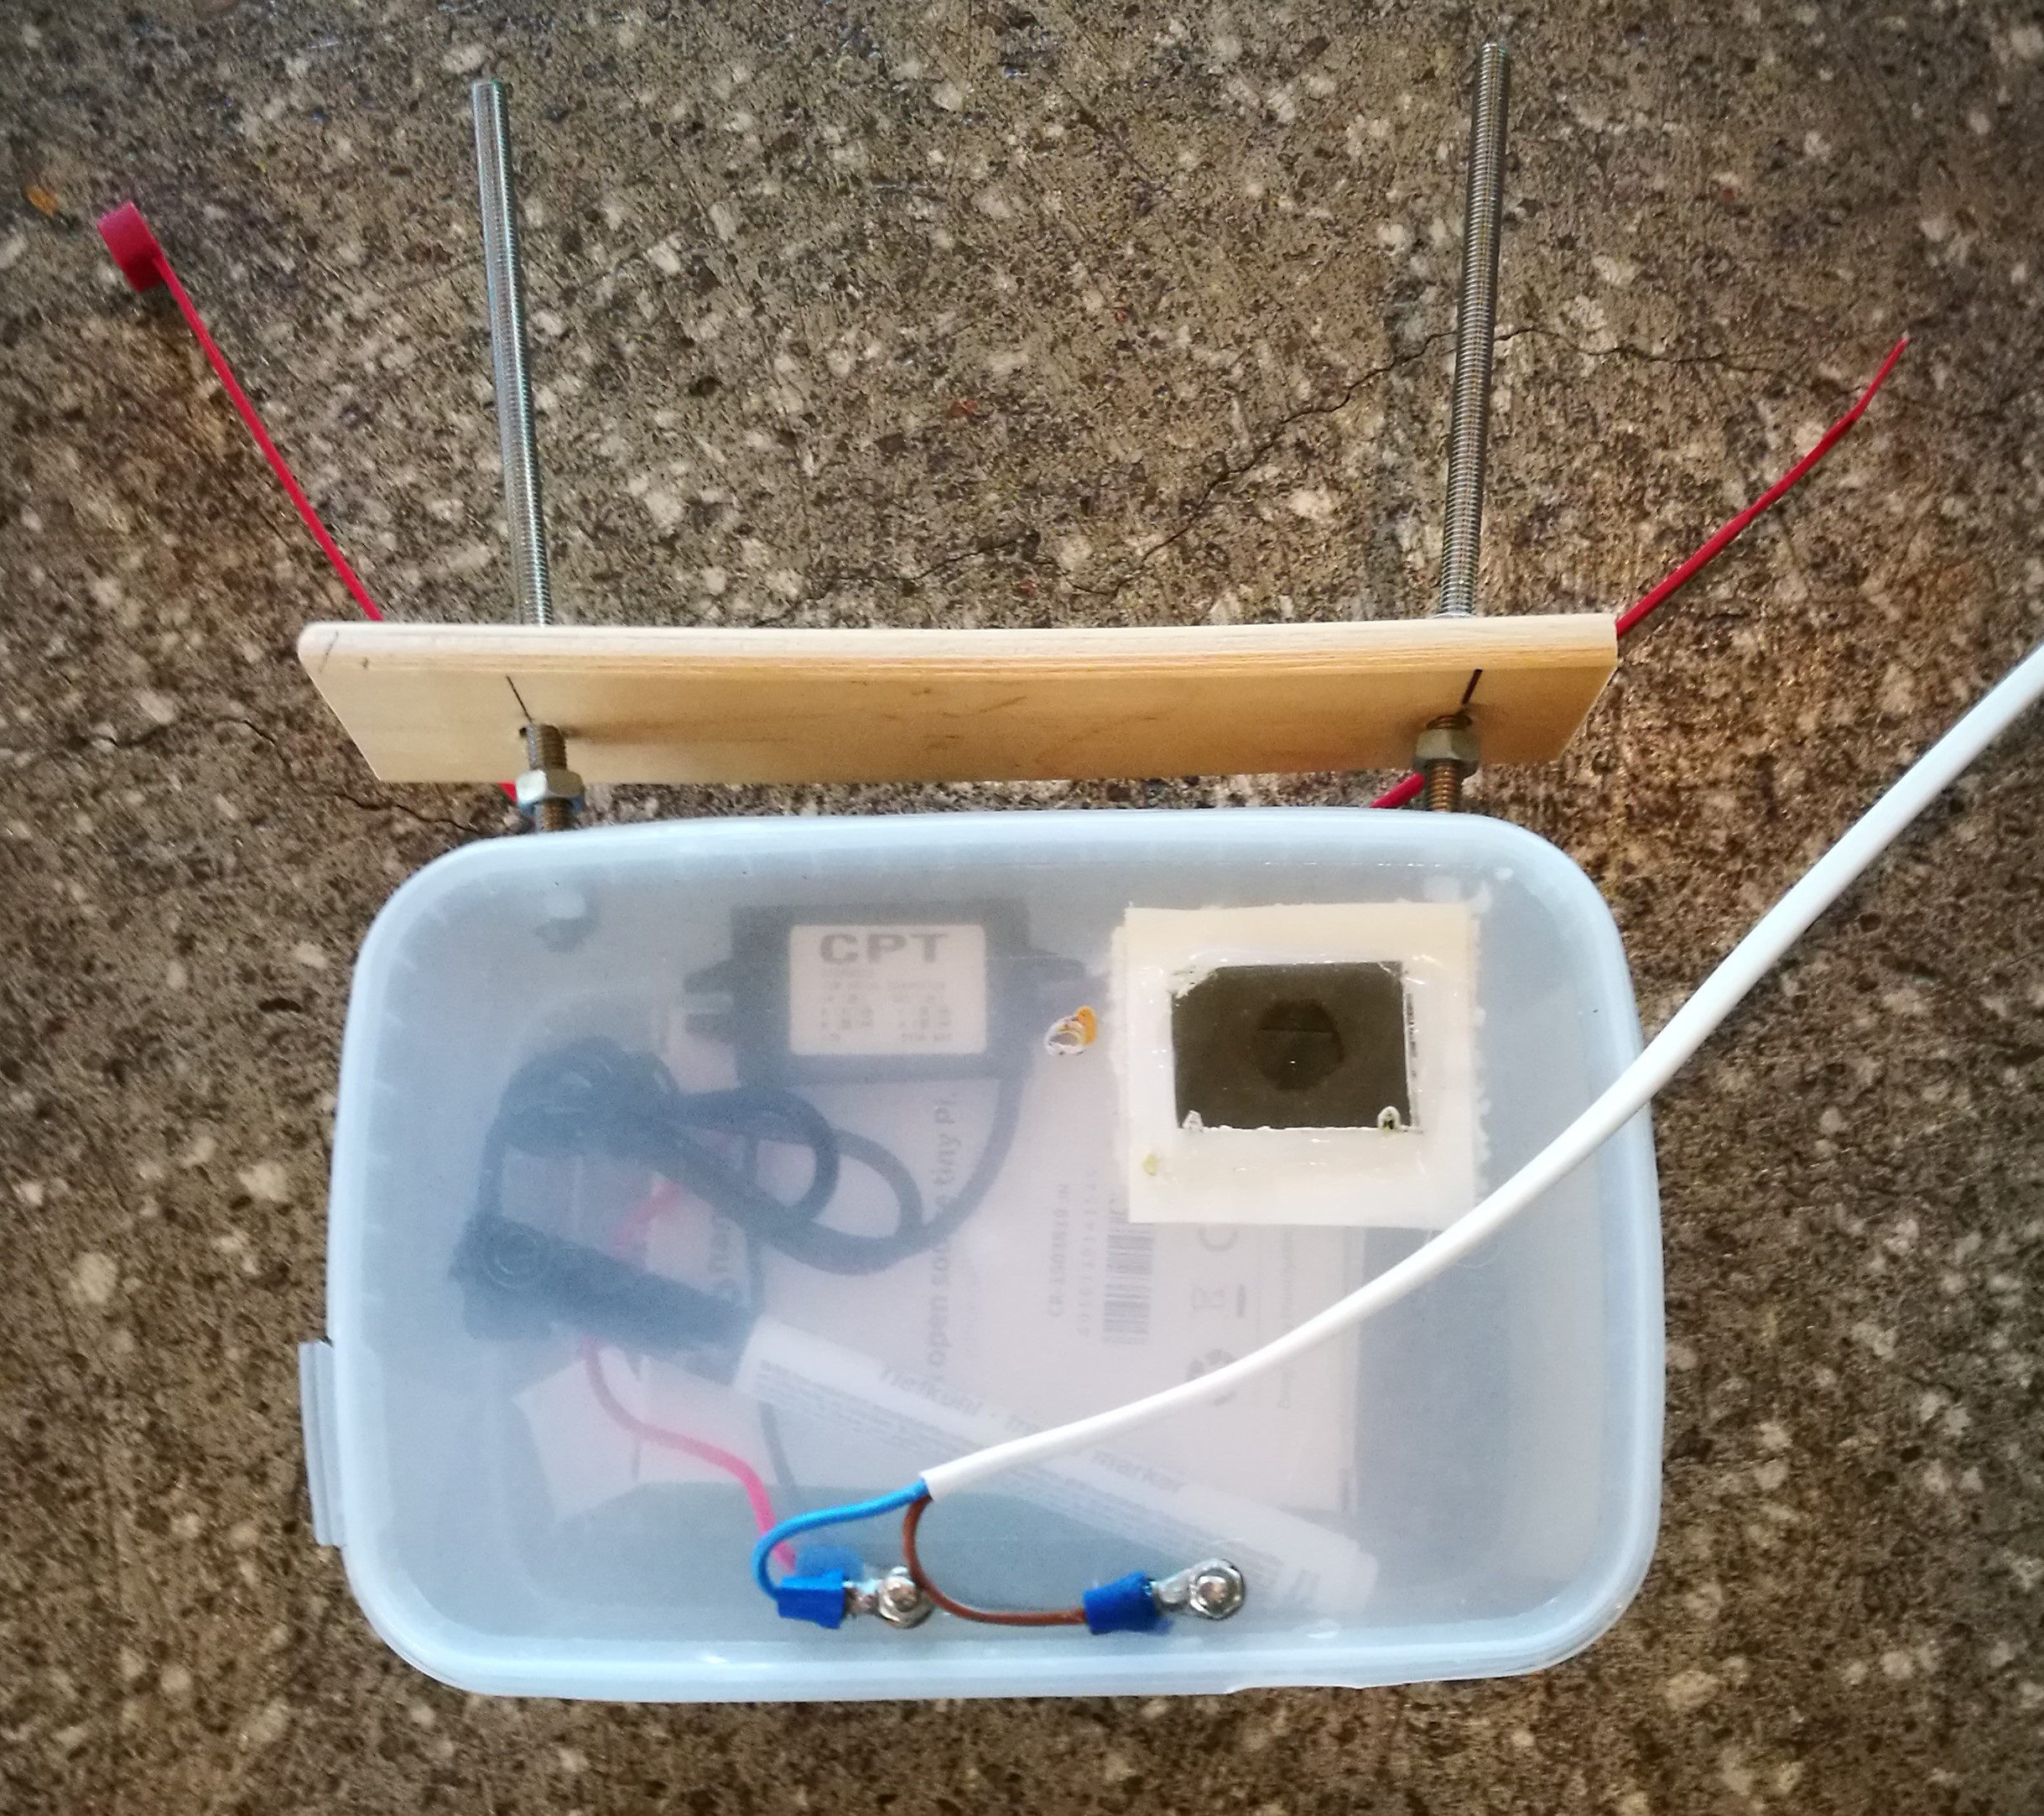
\includegraphics[width=0.5\textwidth]{Hardware/Gehaeuse.jpg} 
  \caption{Foto eines leeren Gehäuses.}
  \label{bGehäuse}
\end{figure}
\newpage
\subsection{Gesamtsystem}
Das Gesamtsystem wurde so günstig wie möglich aufgebaut. Wenn die einzelnen Komponenten bei den preiswertesten Lieferanten bezogen werden, dann kann das gesamte Gerät unter 150 CHF (exkl. Gehäuse) erstellt werden. Die nachfolgende Tabelle (\tref{tKosten}) zeigt eine Auflistung der Kosten des Geräts. Zu den Kleinteilen gehören beispielsweise Schrauben oder Kabel.

\begin{table}[H]
\centering
    \begin{tabular}{p{5cm}l}
    \textbf{Komponente}                & \textbf{Preis}   \\
    NanoPi NEO                         & 10 CHF  \\
    Full HD Kamera                     & 50 CHF  \\
    Autobatterie                       & 50 CHF  \\ 
    WIFI-Adapter                       & 10 CHF  \\
    USB-Hub                            & 5 CHF   \\
    Spannungswandler                   & 10 CHF  \\
    Kleinteile						   & 15 CHF  \\ \hline
    \textbf{Gesamt}                    & \textbf{150 CHF} \\
    \end{tabular}
\caption{Kostenauflistung}
\label{tKosten}
\end{table}

Auf den folgenden Bildern kann das Gesamtsystem betrachtet werden. Dabei ist im ersten Bild ({\fref{bGesamtsystem}) das System in Grossansicht zu sehen, während im zweiten Bild ({\fref{bGesamtsystemH}) das System im Einsatz, hängend an einer Strassenlaterne betrachtet werden kann.

\begin{figure}[H]
  \centering
  
\includegraphics[height=0.6\textwidth]{Hardware/Gesamtsystem.jpg} 
  \caption{Gesamtsystem}
  \label{bGesamtsystem}
\end{figure}

\begin{figure}[H]
  \centering
  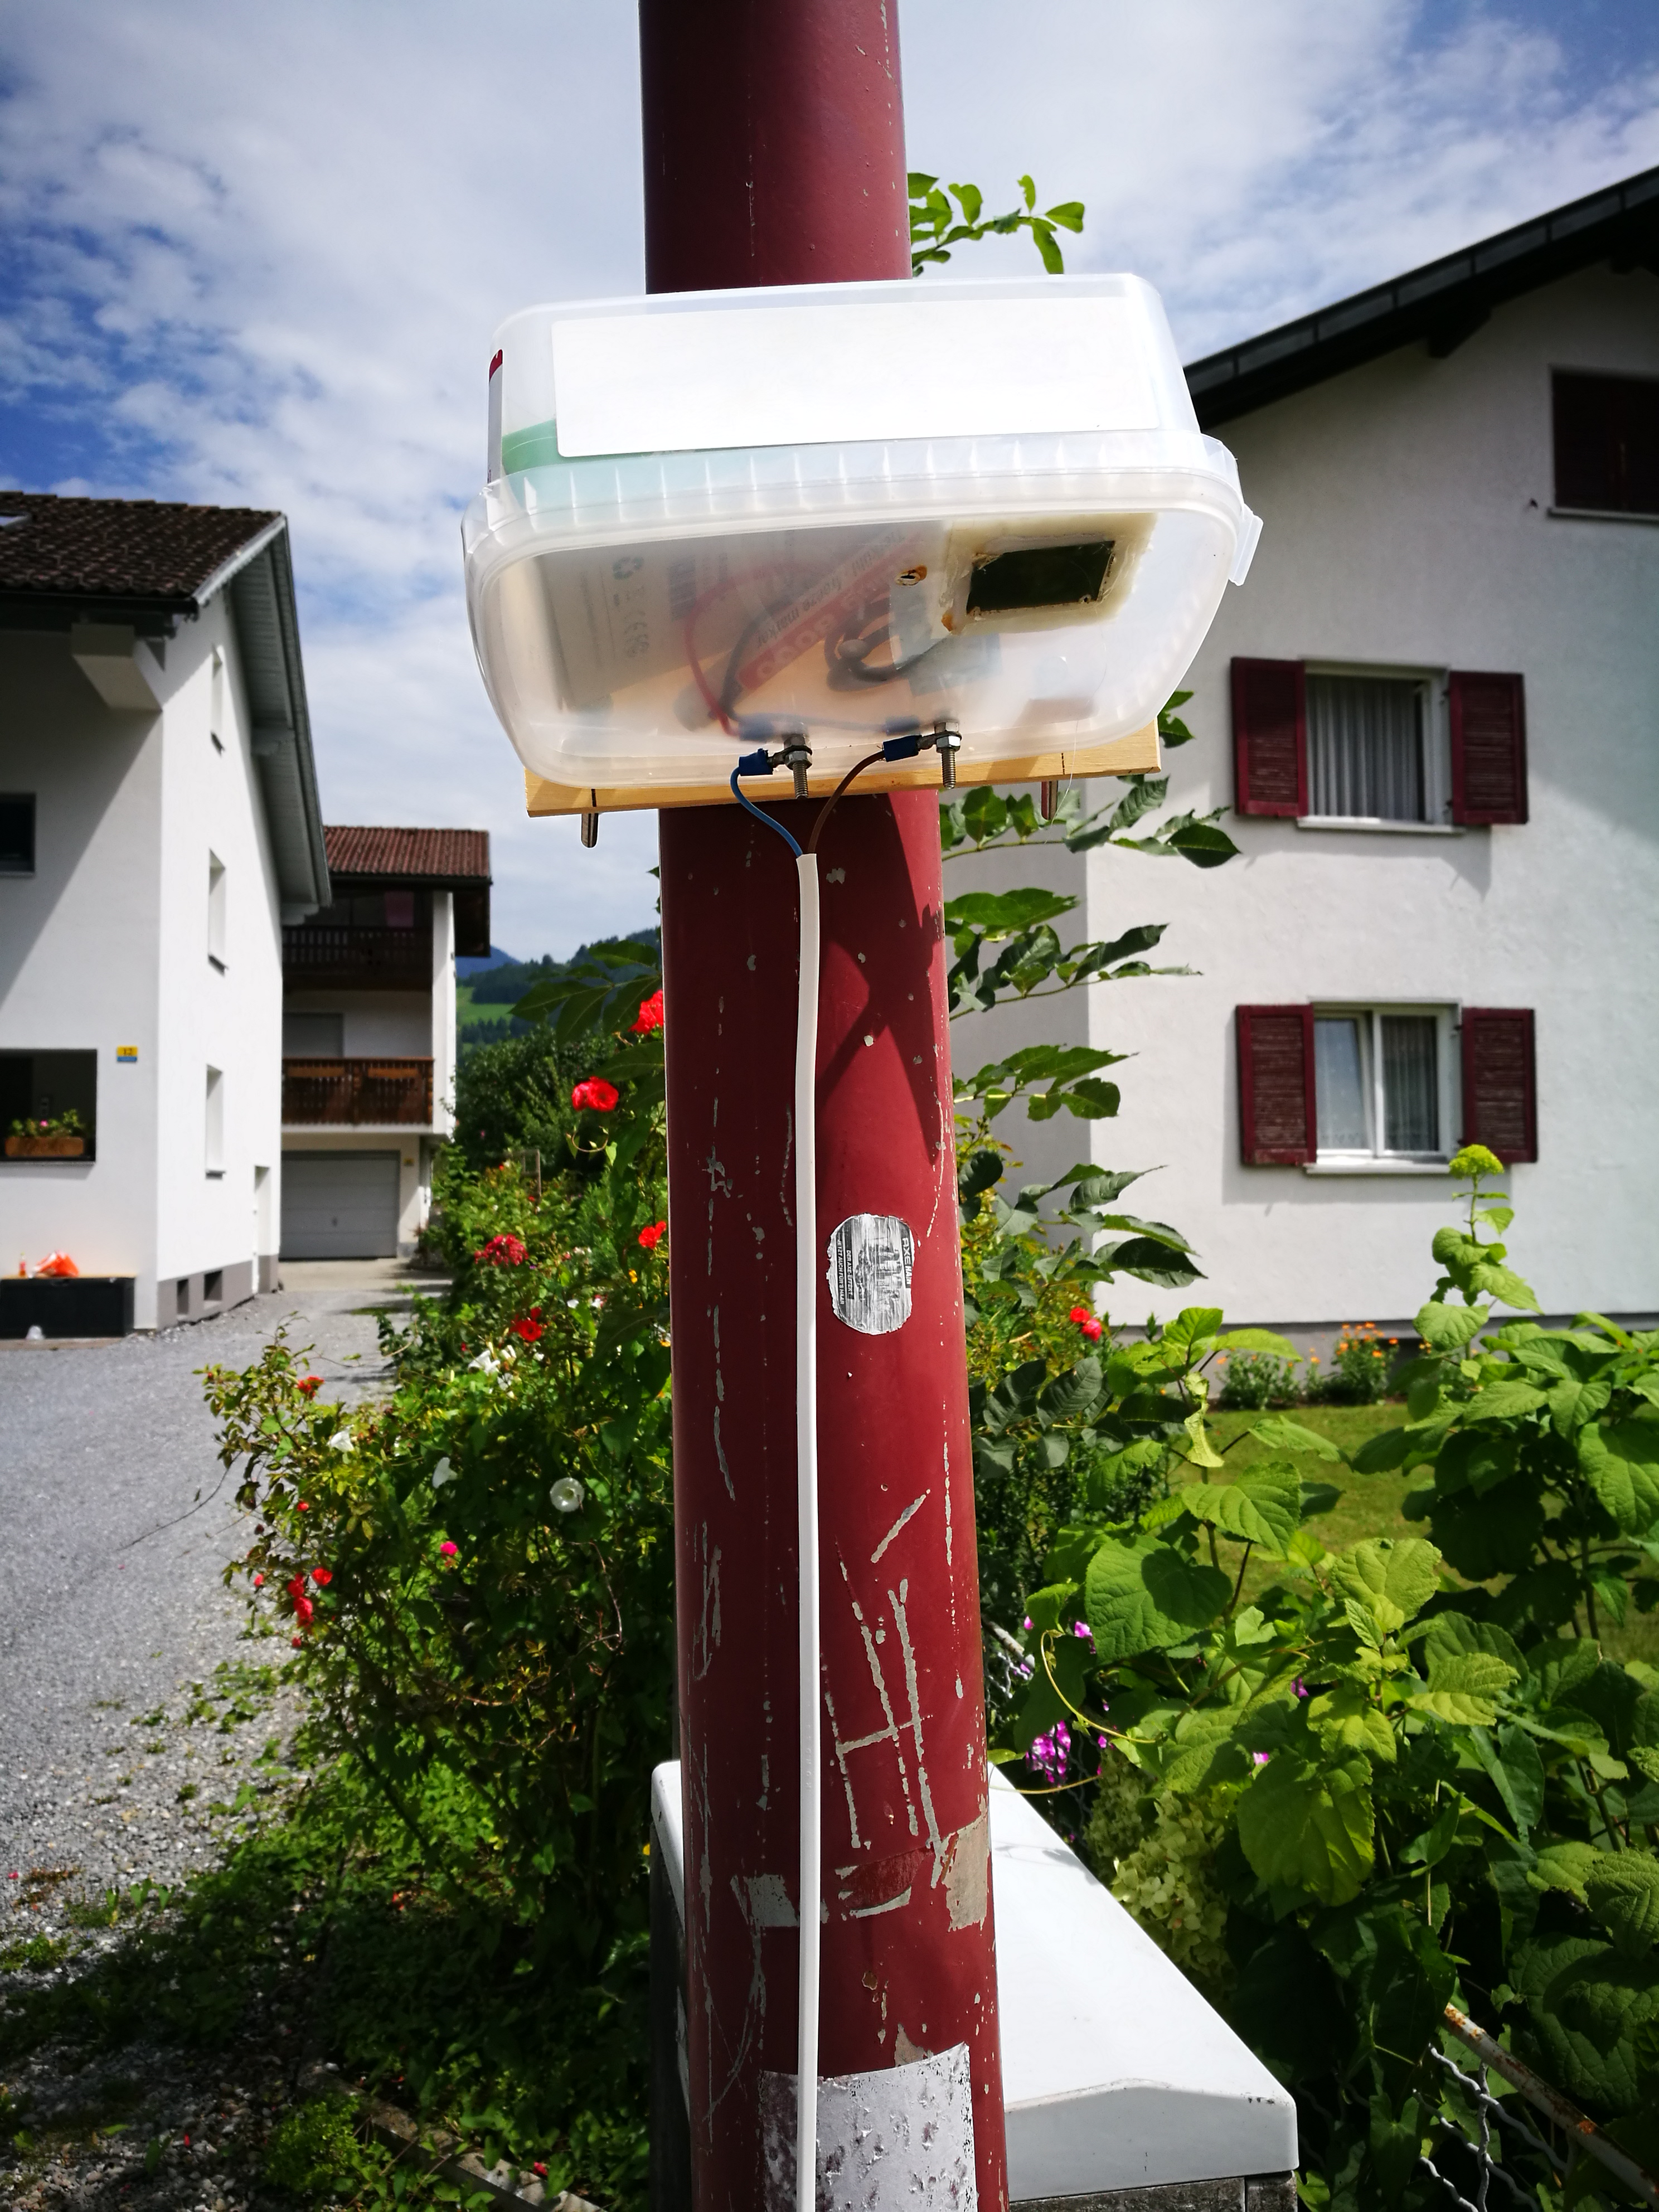
\includegraphics[height=0.6\textwidth]{Hardware/GesamtsystemH.jpg} 
  \caption{Einsatzfähiges Gesamtsystem}
  \label{bGesamtsystemH}
\end{figure}
\newpage
\section{Software}
\subsection{Verwendete Tools und Libraries}
\subsubsection{Mjpg-Streamer}
Beim Mjpg-Streamer handelt es sich um ein Werkzeug für die Kommandozeile, welches ermöglicht Videos von einer Videoquelle aufzunehmen und diese entweder in einer Datei abzuspeichern oder es auf einem Webserver zu streamen. Beim Abspeichern eines Videos konnte etwa eine Bildrate von 15 Bilder pro Sekunde erreicht werden, bevor einige Bilder verloren gingen. \\\\
Grundvoraussetzung für den Mjpg-Streamer ist eine Kamera, welche korrekt eingerichtet wurde. Bei den meisten Modellen muss deshalb der Treiber für "'Video 4 Linux 2"' zuerst installiert werden. Die Installation vom Mjpg-Streamer funktioniert nicht über die offiziellen Paketquellen. Aus diesem Grund müssen zuerst einige andere Pakete der offiziellen Paketquellen installiert werden, bevor der aktuelle Quelltext der eigentlichen Software heruntergeladen und installiert werden kann. Die Verwendung erfolgt relativ simpel, indem zuerst das gewünschte Plugin und danach dessen Parameter übergeben wird. Dies wird sowohl für den Eingang, als auch den Ausgang des Videos benötigt. Einige Parameter für den Eingang der Kamera sind neben dem Plugin auch die Auflösung, der Gerätename, die Bildwiederholrate und die Bildqualität. Bei den Parametern für die Ausgabe handelt es sich um den Speicherort, das Bildintervall oder auch den Port, falls es sich beim Ausgang um einen Webserver handelt. \cite{MjpgStreamer}

\subsubsection{Avconv}
Avconv ist ein sehr schneller Audio- und Videokonverter, welcher dazu verwendet werden kann, um Videos mit Bild und Ton aufzunehmen und diese in einer Datei abzuspeichern. Auch dieses Tool kann von der Kommandozeile aus gesteuert werden und liefert viele Möglichkeiten um Konvertierungen von Bild- und Audiomaterial durchzuführen. Es kann ebenfalls dazu genutzt werden, Videomaterial in andere Datentypen zu konvertieren oder aber Videomaterial schneller beziehungsweise langsamer laufen zu lassen. Avconv bietet beispielsweise die Möglichkeit eine der beiden Spuren auszuschalten, wenn diese nicht benötigt werden. Es können viele Bearbeitungsmöglichkeiten, wie das Schneiden eines Videos in eine gewünschte Länge oder das Verbinden von zwei einzelnen Videos zu einem längeren Video, durchgeführt werden. Ebenso können mehrere Eingänge und Ausgänge angegeben werden, womit es die Möglichkeit bietet, eine eigene Bildspur und Audiospur zu einem Video zu migrieren und es gleichzeitig in mehrere Videoformate abzuspeichern. Anders als beim Mjpg-Streamer kann Avconv direkt von den offiziellen Paketquellen heruntergeladen und installiert werden. Die Verwendung dieses Tools ist komplizierter als beim Mjpg-Streamer, da es viel mehr Parameter beinhaltet. Bei der Videoaufnahme können beispielsweise Parameter wie Auflösung, Eingangsvideogerät, Aufnahmezeit, Bildwiederholungsrate, Bitrate oder Bildqualität angegeben werden. \cite{Avconv}

\subsubsection{OpenCV}
OpenCV ist die Abkürzung für "'Open Source Computer Vision Library"' und ist eine Bibliothek, bei der der Code offen zugänglich und nutzbar ist. Diese Softwarebibliothek ist für Bild- und Videoverarbeitung sowie "'Machine Learning"' und kann in sämtlichen kommerziellen Produkten eingesetzt werden. Die Bibliothek besteht aus mehr als 2500 optimierten Algorithmen und beinhaltet sämtliche gängige Methoden für Bildverarbeitung und "'Machine Learning"'. Zu den Algorithmen gehören beispielsweise das Detektieren und Erkennen von Objekten, Klassifizieren von menschlichen Aktionen, Aufnehmen von Kamerabewegungen, Erkennen von 3D-Objekten und das Produzieren von 3D-Objekten aus einem normalen Kamerabild. Ebenso gehören dazu noch das Zusammenführen von Bildern um hochauflösende Bilder ganzer Szenen zu erschaffen, um ähnliche Bilder in einem Set von Bildern zu finden, rote Augen von Bildern zu entfernen, Verfolgen von Augen oder Gesichtern, "'Augmented Reality"' und vieles mehr. OpenCV bietet Schnittstellen für die Programmiersprachen "'C++"', "'C"', "'Python"', "'Java"' und "'MATLAB"' und unterstützt die gängigen Plattformen Windows, Android, Mac Os und Linux. Es wird stetig weiterentwickelt und kann ohne Probleme in ein Projekt eingebunden werden. Die aktuelle Version ist OpenCV 3.2 und besteht aus Hauptmodulen und Extramodulen. Die normale Installation beinhaltet nur die Hauptmodule, welche jedoch für den normalen Gebrauch ausreichen. Um die Extramodule verwenden zu können, müssen diese zusätzlich heruntergeladen und in den OpenCV Ordner verschoben werden. Für die Installation von OpenCV werden einige offizielle Softwarepakete benötigt, welche man auch vorher herunterladen und installieren muss. Die Installation der neusten Software von OpenCV selber funktioniert nicht über die offiziellen Paketquellen, weshalb die Software manuell heruntergeladen werden muss. \cite{OpenCV}

\subsubsection{Apache}
Unter Apache versteht man bei Linux den "'Apache HTTP Server"'. Dies ist ein sehr bekannter Webserver, welcher meist mit Skriptsprachen, wie PHP, oder Datenbanken, wie MySQL, verwendet wird, um Webseiten zu hosten. Die Installation des "'Apache HTTP Servers"' unter Linux erfolgt lediglich über einen einfachen Befehl und wird dann von den offiziellen Paketquellen heruntergeladen und installiert. Nach der Installation befindet sich der HTTP Server ohne Konfiguration im Autostart und kann nach einem Neustarten der Linux Plattform direkt verwendet werden. Um eigene Internetseiten auf dem Apache zugänglich zu machen, muss die gewünschte Seite als HTML oder PHP in den richtigen Ordner geschoben werden und kann daraufhin über die IP erreicht werden. \cite{Apache}

\subsection{Architektur}
Beim NanoPi Neo handelt es sich, wie bereits erwähnt, um einen Prozessor mit vier Kernen. Dadurch hat man die Möglichkeit vier Prozesse parallel ablaufen zu lassen. Aus diesem Grund wurde in der untenstehenden Abbildung (\fref{bArchitektur}) der Kern symbolisch in vier Abschnitte geteilt, welche die einzelnen Prozesse symbolisieren sollen. Nachfolgend werden die Aufgaben der einzelnen Kerne gezeigt, die schlussendlich das gleichzeitige Aufnehmen und Verarbeiten der Verkehrsteilnehmer ermöglichen.

\begin{figure}[H]
  \centering
  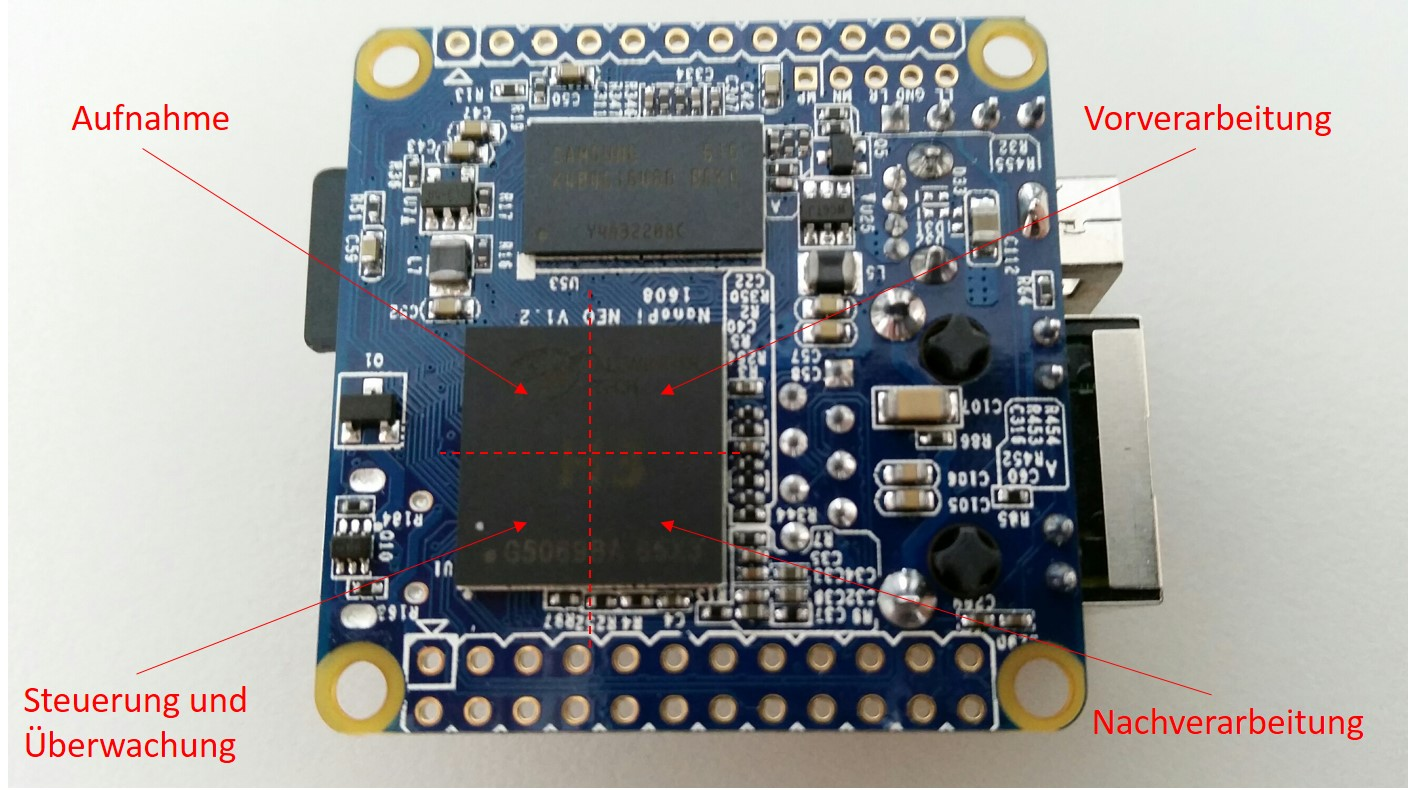
\includegraphics[width=0.99\textwidth]{Software/Architektur.jpg} 
  \caption{Aufteilung der vier Kerne.}
  \label{bArchitektur}
\end{figure}


\subsubsection{Aufnahme}
Der erste Prozess beinhaltet die Aufnahme von Videos mit der Kamera. Die Videos werden mit 25 Bildern pro Sekunde und einer Auflösung von 640x480 Pixeln aufgenommen und auf der Speicherkarte abgelegt. Dabei muss ein Video immer eine Länge von 15 Minuten erzielen, bevor es abgespeichert wird. Die Zeitspanne von 15 Minuten wurde gewählt, damit nach Abschluss dieser Zeit der nächste Prozess sich schon um die Verarbeitung kümmern kann. Währenddessen kann sich der Aufnahmeprozess bereits mit dem nächsten Video beschäftigen. So erreicht man die parallelen Abläufe. Die Videos sind im "'AVI"' Format abgespeichert und beinhalten im Durchschnitt etwa 22'500 Einzelbilder, welche dann vom nachfolgenden Prozess analysiert werden müssen. Mithilfe von Avconv werden diese Videos aufgenommen und mittels Zeitstempel, welcher Datum und Uhrzeit des Aufnahmestarts beinhaltet, im zugehörigen Ordner abgespeichert. Der Zeitstempel wird benötigt um später den Zeitpunkt eines vorbeifahrenden Verkehrsteilnehmers zu errechnen und um zu wissen, welche Videos der Reihe nach weiterverarbeitet werden müssen. Der Prozess der Videoaufnahme ist spezifisch auf den ersten der vier Prozessoren zugeteilt. Während der Aufnahmephase befindet sich dieser Kern stetig bei einer Auslastung von 95 - 100\%.

\subsubsection{Vorverarbeitung}
Sobald sich zwei Videos im dafür vorgesehenen Ordner befinden, kann davon ausgegangen werden, dass die Aufnahme des ersten Videos abgeschlossen ist. Zu diesem Zeitpunkt beginnt die Vorverarbeitung damit, die Bilder zu analysieren und diese, sobald eine Bewegung auf dem Bild erkannt wurde, in einen separaten Ordner abzuspeichern, welcher extra für diese Frames genutzt wird. Da die Videoaufnahme innerhalb von 15 Minuten jeweils 22'500 Bilder erzeugt, muss die Vorverarbeitung etwa gleich viel Bilder in der selben Zeit auswerten können. Aus diesem Grund wurde das Programm für diesen Prozess soweit optimiert, dass nur sehr wenig einzelne Schritte durchgeführt werden müssen. Diese Analyse wird mithilfe der Bildverarbeitungsbibliothek OpenCV durchgeführt. Dabei kann ein Video angegeben werden, woraufhin von diesem das nächste nicht genutzte Frame in einer temporären Variablen gespeichert wird. Mit diesen Variablen können im Anschluss weitere Berechnungen durchgeführt werden. Die Vorverarbeitung nimmt jeweils zwei aufeinanderfolgende Frames und subtrahiert bei diesen Bildern jedes einzelne Pixel an derselben Stelle voneinander ab. Falls es keine Bewegung beim spezifischen Pixel gab, so ergibt die Subtraktion der Pixel an dieser Stelle den Wert Null. Der Pixel erscheint auf diesem Bild dann schwarz. Falls sich jedoch Bewegungen abgespielt haben, ergibt diese Berechnung einen höheren Wert und es erscheint auf dem Bild heller bzw. farbig. Dies wird für jedes der 640x480 Pixel in einem Bild durchgeführt. Daraufhin werden im nächsten Schritt die erhaltenen Differenzen addiert. Folglich erhält man eine Zahl, welche die Gesamtsumme aller Differenzen dieser 307'200 einzelnen Pixel repräsentiert. Diese Zahl ist schlussendlich ausschlaggebend für eine allfällige Bewegung zwischen diesen beiden Bildern. Die nachfolgende Abbildung (\fref{bFrames}) zeigt zwei aufeinanderfolgende Frames.

\begin{figure}[H]
  \centering
  \subfigure[Frame1]{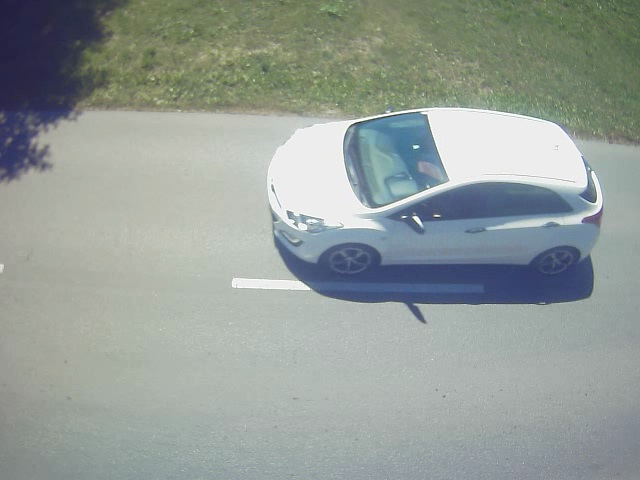
\includegraphics[width=0.49\textwidth]{Software/Frame1.jpg}}
  \subfigure[Frame2]{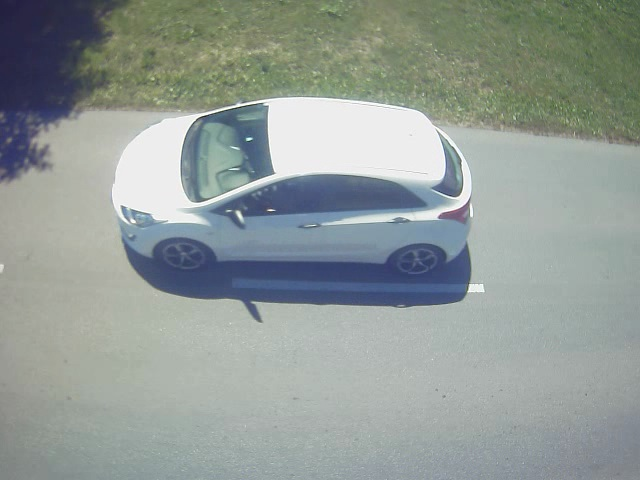
\includegraphics[width=0.49\textwidth]{Software/Frame2.jpg}}
  \caption{Zwei aufeinanderfolgende Frames}
  \label{bFrames}
\end{figure}

Anschliessend wurde die oben erwähnte Berechnung mit diesen beiden Frames durchgeführt, wodurch Bewegungen zwischen den Bildern heller bis farbig erscheinen. Das Ergebnis der Subtraktion ist im folgenden Bild (\fref{bBlur1}) ersichtlich.

\begin{figure}[H]
  \centering
  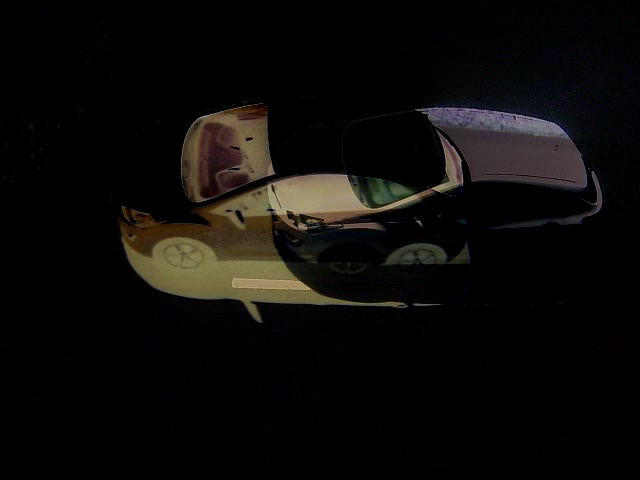
\includegraphics[height=0.3\textheight]{Software/Blur1.jpg} 
  \caption{Differenzbild der aufeinanderfolgenden Frames.}
  \label{bBlur1}
\end{figure} 

Damit ein allfälliges Rauschen oder ein vorbeilaufender Fussgänger nicht erfasst wird, wurde ein gewisser Schwellwert angegeben. Sobald die Summe der Pixel den Schwellwert überschreitet, wird das Bild temporär abgespeichert. Damit die Bilder im nächsten Schritt logisch verknüpft werden können, muss im Speichername eine Indexierung angegeben werden. Diese Indexierung ist die Zahl des Frames, welches vom Video stammt und liegt aus diesem Grund zwischen 0 und 22'499. Falls keine Speicherung stattgefunden hat wird das nächste Bild genommen und der Vorgang beginnt erneut. Mit dieser Methode werden etwa 25 Bilder pro Sekunde verarbeitet. Da jedoch für das Abspeichern der Bilder mehr Zeit benötigt wird als für das Verwerfen, können bei höherem Verkehrsaufkommen nur etwa 20 Einzelbilder verarbeitet werden. Nachdem ein komplettes Video abgearbeitet wurde, wird es aus Platzgründen und weil es für den weiteren Verlauf der Auswertung nicht mehr benötigt wird gelöscht. Dies ist die letzte Aufgabe der Vorbearbeitung. Von den 22'500 Einzelbildern, die von diesem Prozess bearbeitet wurden, sind zu diesem Zeitpunkt, je nach Verkehrsaufkommen, noch etwa 500 - 1'500 Bilder im Zwischenspeicher. Sie werden dann vom nächsten Prozess, der Nachverarbeitung, weiterbearbeitet. Da die Vorverarbeitung sehr viel Leistung erbringen muss, wurden ihm die Prozessorkerne zwei und vier zugeteilt. Die Steuerung und Überwachung, welche fix auf dem vierten Prozessorkern liegt, benötigt nur eine geringe Auslastung. Aufgrund dessen kann der Prozess der Vorverarbeitung die zwei Kerne beinahe voll auslasten, um somit die vielen Einzelbilder möglichst effizient verarbeiten zu können.

\subsubsection{Nachverarbeitung}
Nachdem die Vorverarbeitung ein Video analysiert und die relevanten Frames abgespeichert hat, kann die Nachverarbeitung beginnen. Auch hier, wird der Prozess erst gestartet, wenn sich zwei unterschiedliche Ordner mit Frames im zugehörigen Ordner befinden. Somit soll gewährleistet sein, dass die Vorverarbeitung mit dem Video fertig ist, bevor die Nachverarbeitung mit dem Prozess beginnt. Das Endprodukt der Nachbearbeitung ist ein Feature Vektor. Dies ist eine Microsoft Excel Tabelle mit je einem Eintrag pro Verkehrsteilnehmer. Dabei werden möglichst viele Indikatoren pro Verkehrsteilnehmer aufgenommen und in der Tabelle abgespeichert. Je mehr Features pro Fahrzeug gefunden werden können, desto besser kann dieses später wiedererkannt werden und die eigentliche Verkehrsverfolgung durchgeführt werden. Nachfolgende Tabelle (\tref{tFeatureVektor}) zeigt ein Beispiel eines Feature Vektors.

\setlength\tabcolsep{5pt}

\begin{table}[H]
\centering
\begin{tabular}{|l|l|l|l|l|l|l|l|l|l|l|l|}
\hline
\textbf{I} & \textbf{Timestamp}  & \textbf{RP} & \textbf{D} & \textbf{DC} & \textbf{CropN} & \textbf{BlurN} & \textbf{PicN} & \textbf{RX} & \textbf{RY} & \textbf{RW} & \textbf{RH} \\ \hline
1            & 18.06.17 22:55:12 & 5           & R            & 1           & crop001.tif       & blur001.tif       & pic001.tif       & 95          & 141         & 377         & 190         \\ \hline
2            & 18.06.17 22:57:19 & 8           & R            & 2           & crop002.tif       & blur002.tif       & pic002.tif       & 146         & 118         & 387         & 196         \\ \hline
3            & 18.06.17 22:57:37 & 7          & L            & 1           & crop003.tif       & blur003.tif       & pic003.tif       & 138         & 145         & 373         & 251         \\ \hline
4            & 18.06.17 22:58:10 & 7           & R            & 3           & crop004.tif       & blur004.tif       & pic004.tif       & 152         & 112         & 345         & 165         \\ \hline
5            & 18.06.17 22:59:02 & 6           & L            & 2           & crop005.tif       & blur005.tif       & pic005.tif       & 115         & 126         & 415         & 296         \\ \hline
6            & 18.06.17 22:59:23 & 5           & R            & 4           & crop006.tif       & blur006.tif       & pic006.tif       & 145         & 126         & 364         & 194         \\ \hline
7            & 18.06.17 22:59:56 & 5          & R            & 5           & crop007.tif       & blur007.tif       & pic007.tif       & 113         & 100         & 453         & 311         \\ \hline
8            & 18.06.17 22:59:59 & 9           & R            & 6           & crop008.tif       & blur008.tif       & pic008.tif       & 165         & 138         & 358         & 182         \\ \hline
9            & 18.06.17 23:00:09 & 9           & L            & 3           & crop009.tif       & blur009.tif       & pic009.tif       & 148         & 160         & 367         & 212         \\ \hline
10           & 18.06.17 23:00:18 & 7           & R            & 7           & crop010.tif       & blur010.tif       & pic010.tif       & 147         & 127         & 371         & 198         \\ \hline
11           & 18.06.17 23:00:37 & 4           & R            & 8           & crop011.tif       & blur011.tif       & pic011.tif       & 155         & 128         & 341         & 189         \\ \hline
\end{tabular}
\caption{Feature Vektor}
\label{tFeatureVektor}
\end{table}

\setlength\tabcolsep{0pt}

Der Feature Vektor zeigt den Index anhand einer fortlaufenden Nummer und den Zeitstempel, an welchem sich der Verkehrsteilnehmer in etwa in der Mitte des Kamerabildes befand. Ebenso enthält er die Information wie viele aufeinanderfolgende Bilder zu diesem Ergebnis geführt haben, in welche Richtung der entsprechende Verkehrsteilnehmer unterwegs war und einen Zähler der sowohl für links- als auch rechtsfahrende Fahrzeuge stetig erhöht wird. Daneben werden im Moment noch drei Bilder abgespeichert, welche für weitere Berechnungen von Features benützt werden können. Die letzten vier Spalten zeigen die Position des Verkehrsteilnehmers im Originalbild.\\\\
Die Nachverarbeitung kümmert sich in erster Linie darum, den Feature Vektor zu öffnen, falls dieser vorhanden ist, um daraus relevante Informationen zu entnehmen. Ist der Feature Vektor nicht vorhanden, so wird ein neuer generiert. Zu den relevanten Informationen gehört ein Index. Dieser ist notwendig, damit im Feature Vektor kein Index doppelt vorkommt und somit bereits vorhandene Bilder überschrieben werden. Zudem wird die Anzahl an Verkehrsteilnehmer, welche bis zu diesem Zeitpunkt nach links bzw. rechts gefahren sind, in einer Variablen gespeichert. Diese beiden Zähler können weiter erhöht werden, wenn neue Verkehrsteilnehmer erkannt werden. Dies ist erforderlich, da sich dieses Programm nach Abarbeitung der Frames beendet und somit alle bestehenden Informationen verliert. Anschliessend wird die Anzahl der relevanten Bilder ermittelt, welche zu einem Verkehrsteilnehmer gehören. Dies passiert, indem die Frames genommen und deren Indexierungen betrachtet werden. Falls die Indexierungen der Frames fortlaufend sind, so muss es sich zwangsläufig um denselben Verkehrsteilnehmer handeln. Falls der Abstand zwischen zwei Frames einen gewissen Wert überschreitet, hat die Kamera für kurze Zeit keine Bewegung erkannt. Folglich muss es sich dann um einen neuen Verkehrsteilnehmer handeln. Sobald die Zahl der relevanten Bilder bekannt ist, werden diese logisch miteinander verknüpft.\\\\
Aus diesen etwa drei bis zehn Bildern, je nach Geschwindigkeit des Fahrzeugs, wird nun mit der Bildverarbeitungsbibliothek OpenCV ein "'Blob Detection"' mit anschliessendem "'Blob Tracking"' durchgeführt. Zuerst werden Bewegungen zwischen zwei aufeinanderfolgenden Bildern ermittelt und dann um die Pixel in der unmittelbaren Umgebung eine konvexe Hülle, die auch Blob genannt wird, gebildet. Auf den fortlaufenden Bildern wird sich diese konvexe Hülle immer weiter zum Rand bewegen. Im Programm selbst wurde festgelegt, welche Voraussetzungen erfüllt werden müssen, damit dieser Blob als Verkehrsteilnehmer gezählt wird. Dazu gehören die Fläche der Hülle, das Verhältnis zwischen Länge und Breite, die minimale Breite und Länge und die minimale Länge der Diagonale. Falls es sich beim Blob um einen Verkehrsteilnehmer handelt, muss noch ermittelt werden, zu welchem Zeitpunkt dieser die Mitte passiert und somit die Bilder generiert werden müssen. Dies wird mithilfe einer imaginären Linie durchgeführt, welche sich in der Mitte des Bildes befindet. Da die Position des Blobs von Anfang an bekannt ist, kann auch ermittelt werden, ob der Verkehrsteilnehmer von links nach rechts oder von rechts nach links gefahren ist.\\\\
Die nachfolgenden Abbildungen (\fref{bMotionDetection}) zeigen ein Auto, welches, von rechts nach links fahrend, von der Kamera mit drei Frames aufgenommen wurde. Da dieses Auto alle festgelegten Parameter erfüllt, wird es als Verkehrsteilnehmer erkannt und eine konvexe Hülle gebildet. Die konvexe Hülle wird immer um zwei nachfolgende Frames gebildet, weshalb diese bei sämtlichen Bildern länger als der entsprechende Verkehrsteilnehmer ist. Im ersten und zweiten Frame befindet sich die Mitte der konvexen Hülle und damit auch die Mitte des gelben Quadrats jeweils auf der rechten Seite der Linie. Zu diesem Zeitpunkt wurde noch keine Zählung durchgeführt. Erst beim dritten Frame hat die Mitte des Blobs die rote Linie überquert. Dadurch wurde die Funktion zum Abspeichern eines Fahrzeugs und generieren einer neuen Zeile im Feature Vektor ausgelöst.

\begin{figure}[H]
\centering
	\subfigure[Blob Frame 1]{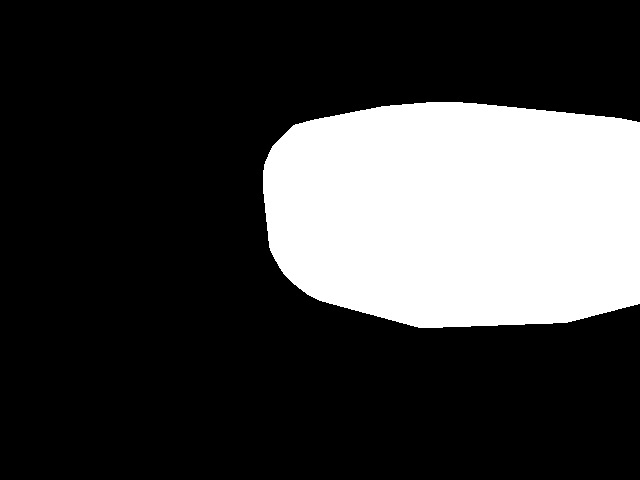
\includegraphics[width=0.48\textwidth]{Software/Blob1.jpg}}\quad
   \subfigure[Bild Frame 1]{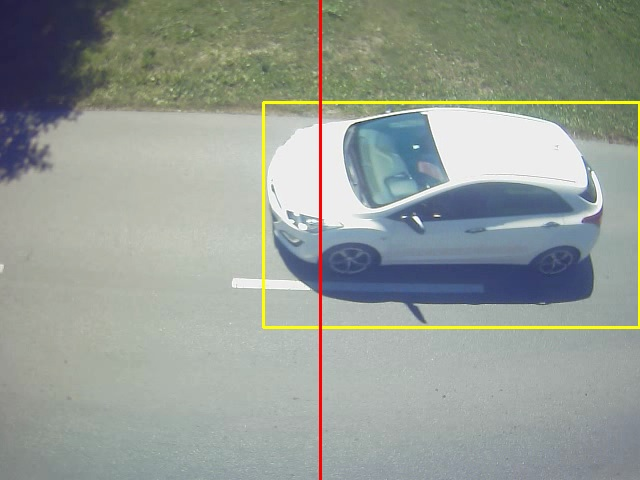
\includegraphics[width=0.48\textwidth]{Software/Detection1.jpg}}\\
   \subfigure[Blob Frame 2]{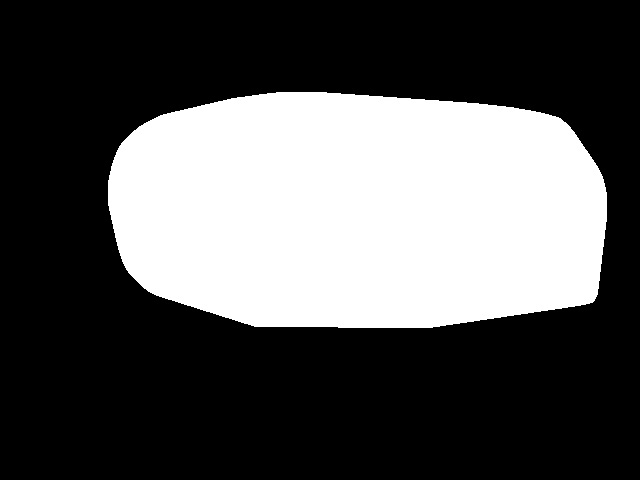
\includegraphics[width=0.48\textwidth]{Software/Blob2.jpg}}\quad
   \subfigure[Bild Frame 2]{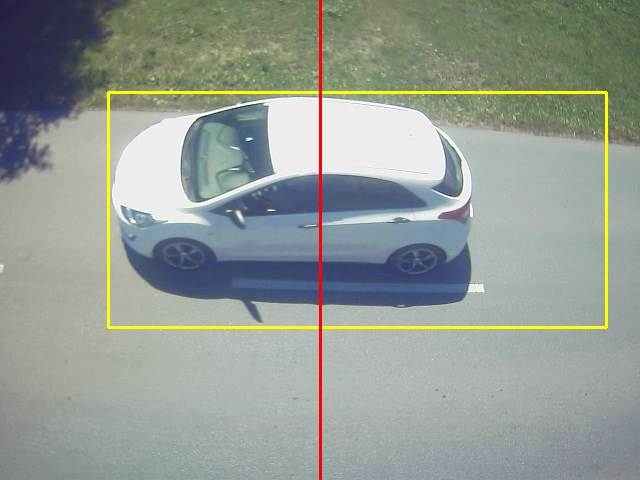
\includegraphics[width=0.48\textwidth]{Software/Detection2.jpg}}\\
   \subfigure[Blob Frame 3]{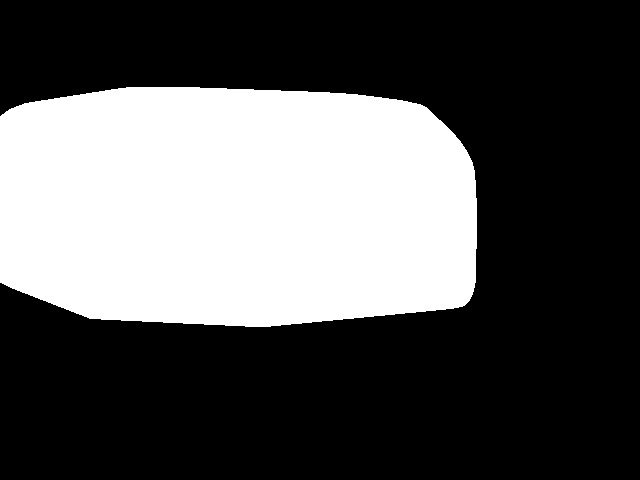
\includegraphics[width=0.48\textwidth]{Software/Blob3.jpg}}\quad
   \subfigure[Blob Frame 3]{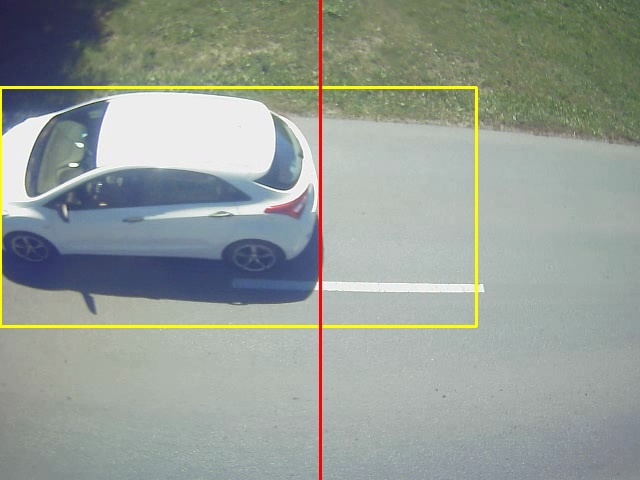
\includegraphics[width=0.48\textwidth]{Software/Detection3.jpg}}
\caption{Vehicle Tracking mithilfe von Blobs}
\label{bMotionDetection}
\end{figure}

Die drei vorher erwähnten Bilder werden in den entsprechenden Ordnern im Speicher abgelegt und alle relevanten Informationen an den Filehandler übergeben. Dieser öffnet die Datei des Feature Vektors und schreibt alle Informationen inklusive berechnetem Zeitstempel in eine neue Zeile. \\\\
Nach diesem Vorgang ist der Verkehrsteilnehmer erfolgreich aufgenommen und abgeschlossen. Der nächste Teilnehmer kann nun ermittelt werden.\\\\
Wenn sich keine Bilder mehr im Frames-Ordner befinden, beginnt die letzte Aufgabe dieses Programms. Der bereits bearbeitete Ordner wird gelöscht, da auch dieser für die weitere Auswertung nicht mehr benötigt wird. Der Nachbearbeitung wurde fix der dritte Prozessorkern zugeteilt. Bei hohem Verkehrsaufkommen benötigt diese auch die vollen 100\% dieses Kerns.\\\\
Diese Software basiert auf dem Grundgerüst von \cite{OpenCVCC} und wurde an die Aufgaben von "'Fast and Curious"' angepasst, verändert und erweitert.

\subsubsection{Steuerung und Überwachung}
Vorhin wurde bereits erwähnt, dass sich die Prozesse selber beenden, sobald sie ihre Arbeit erledigt haben. Folglich wird ein Prozess benötigt, der sich hauptsächlich um die gesamte Koordination kümmert. Videos werden nur zwischen morgens um 05:00 Uhr und abends um 21:00 Uhr aufgenommen. Dies ist notwendig um sicherstellen zu können, dass alle Videos bis zum nächsten Morgen bearbeitet wurden. Dadurch soll ein Speicherplatzproblem verhindert werden, falls die Vorverarbeitung aufgrund eines hohen Verkehrsaufkommens die Videos langsamer prozessiert als diese aufgenommen werden.\\\\
Die Steuerung und Überwachung ist so konzipiert, dass sie ständig eine Schleife von Befehlen durchläuft. Die erste Aufgabe besteht darin den aktuellen Zeitpunkt zu kontrollieren. Falls die Nachtphase noch nicht aktiv ist wird im nächsten Schritt geprüft, ob der Prozess zur Videoaufnahme noch läuft. Dadurch kann sofort ein neuer Prozess zur Aufnahme gestartet werden, falls kein Video mehr aufgenommen wird.\\\\
Als nächstes wird die Anzahl der Videos im dazugehörigen Ordner kontrolliert und anschliessend auch hier der Prozess zur Vorverarbeitung analysiert. Wenn die Vorverarbeitung nicht läuft, muss diese neu gestartet werden. Dazu wird jedoch der Pfad zum Video benötigt, welches als nächstes bearbeitet werden muss. Aus diesem Grund muss es möglich sein den Pfad anhand des Erstellungsdatums der Videos herauszulesen. Danach kann die Vorverarbeitung mit dem dazugehörigen Pfad des Videos gestartet werden.\\\\
Nach dem gleichen Konzept geht es auch beim dritten Prozess, der Nachbearbeitung, weiter. Der einzige Unterschied zwischen dem zweiten und dritten Prozess besteht darin, dass hierfür zum Starten der Pfad zum Ordner mit den Frames benötigt wird.\\\\
Da nebenbei noch ein Webserver läuft, der Informationen bereitstellt, wenn man sich mit dem "'Fast and Curious"'-Gerät verbindet, hat die Steuerung und Überwachung noch kleinere Aufgaben für besagten Server. Dies bedeutet, auf Eingaben der Website zu reagieren und Ordner zu erstellen oder zu verschieben, wenn dies vom Benutzer gewünscht wird. Zudem ist eine Temperaturüberwachung eingebaut. Einmal pro Minute wird die Kerntemperatur ausgelesen und in ein File geschrieben. Diesem Prozess ist der vierte Prozessorkern zugeteilt. Da die Auslastung des Scripts jedoch nicht sonderlich hoch ist, teilt sich dieser Prozess den Kern mit der Vorverarbeitung. \cite{Bash}

\subsection{Github}
Zur Verwaltung der Software wurde Github verwendet. Damit konnten Anpassungen oder Änderungen des Quellcodes einfach von der Komandozeile, im Webbrowser oder mithilfe eines Programms unter Windows hochgeladen und anschliessend auf anderen Geräten verbreitet werden. Ebenfalls war es jederzeit möglich die Software auf vorherige Versionen des Quellcodes zurückzusetzen, wenn dies notwendig war. Durch "'Sourcetree"', einem Programm unter Windows, konnten zudem sämtliche vorgängige Commits rasch und einfach nachgelesen und nachvollzogen werden, da dort zu jedem Commit die spezifischen Änderungen markiert wurden. Ein weiterer Vorteil von Github war es, dass der Quellcode von überall aus erreichbar war, und somit keine verschiedenen Versionen von Codes vorhanden waren. Da der Code jederzeit und überall erreichbar war, konnte dies im späteren Verlauf der Bachelorarbeit, als die Geräte bereits an den Strassenlaternen angebracht waren, verwendet werden um den Quellcode stetig zu verbessern. Neue Versionen der Software konnten anschliessend per WLAN heruntergeladen und installiert werden, wobei die Geräte nicht entfernt und neu ausgerichtet werden mussten. So konnte der Quellcode jederzeit getestet, angepasst und innerhalb weniger Minuten auf den Geräten aktualisiert werden. Das Update konnte mittels eines Scripts durchgeführt werden, welches für sämtliche Programme unter Linux zuerst eine Überprüfung durchgeführt hatte, ob das gewünschte Programm bereits installiert war und neue Software nur installierte, falls diese nicht auf dem Board vorhanden waren. So konnte die Installationszeit für Updates sehr kurz gehalten werden.

\subsubsection{Ordnerstruktur}
Sämtlicher Quellcode, welcher auf dem Gerät installiert wurde, ist unter nachfolgendem Link verfügbar. In der untenstehenden Tabelle (\tref{tOrdnerstruktur}) sind die wichtigsten Dokumente und Ordner des Quellcodes aufgelistet und deren Verwendungszweck anschliessend kurz erklärt:\\

\url{https://github.com/josef94/BA}\\

\setlength\tabcolsep{5pt}

\begin{table}[H]
\centering
\begin{tabular}{|p{0.2 cm}|p{3.5 cm} p{3.5 cm} p{3.5 cm}|}
\hline
\multicolumn{4}{|l|}{\textbf{MakeVideo}} \\ \hline
 & makeVideo.sh &  &  \\ \hline
\multicolumn{4}{|l|}{\textbf{CheckMotion}} \\ \hline
 & CheckMotion.cpp &  &  \\ \hline
 \multicolumn{4}{|l|}{\textbf{VehicleCount}} \\ \hline
 & \begin{tabular}[c]{@{}l@{}}Blob.cpp\\ Blob.h\end{tabular} & \begin{tabular}[c]{@{}l@{}}FileHandler.cpp\\ FileHandler.h\end{tabular} & VehicleCount.cpp \\ \hline
\multicolumn{4}{|l|}{\textbf{Handler}} \\ \hline
 & handler.sh & settings.sh & temperature.sh \\ \hline
\multicolumn{4}{|l|}{\textbf{WLAN}} \\ \hline
 & WLANSettings.sh &  &  \\ \hline
\multicolumn{4}{|l|}{\textbf{Temp}} \\ \hline
 & \begin{tabular}[c]{@{}l@{}}deleteFrames.sh\\ generateCrops.sh\\ generateFeatureVec.sh\end{tabular} & \begin{tabular}[c]{@{}l@{}}index.php\\ rc.local\\ startStream.sh\end{tabular} & \begin{tabular}[c]{@{}l@{}}startVideo.sh\\ temperature.php\end{tabular} \\ \hline
\multicolumn{4}{|l|}{} \\ \hline
 & initialization.sh &  &  \\ \hline
\end{tabular}
\caption{Ordnerstruktur Github.com/josef94/BA}
\label{tOrdnerstruktur}
\end{table}

\setlength\tabcolsep{0pt}

Das Skript "'makeVideo.sh"' dient dazu, die Videoaufnahme zu starten. Nach Aufruf des Scripts, wird ein Zeitstempel mit aktuellem Datum und Uhrzeit herausgelesen und daraufhin ein 15-Minütiges Video gestartet, welches im Videos-Ordner gespeichert wird.\\

Die C++ Datei CheckMotion ist für die Vorverarbeitung zuständig. Nachdem die Datei kompiliert wurde, kann diese ausgeführt werden. Dieses Programm benötigt jedoch den Namen des Videos und den Pfad für die generierten Frames als Argument.\\

Sämtliche Dateien im VehicleCount werden benötigt, um die Nachbearbeitung durchzuführen. Auch diese Dateien müssen vorgängig kompiliert werden, damit sie ausführbar sind. Dabei ist VehicleCount die Hauptklasse, Filehandler kümmert sich um das Datei-Handling und Blob um die eigentliche "'Blob-Detection"'. Als Argument benötigt die Hauptklasse den korrekten Pfad des Ordners.\\

Die drei Dateien im Ordner "'Handler"' gehören zur Steuerung und Überwachung. Dabei beinhaltet die Datei "'handler.sh"' die Hauptschleife. "'settings.sh"' wird benötigt, um den Life-Stream zu starten, damit das Gerät ausgerichtet werden kann und "'temperature.sh"' liest alle 60 Sekunden die Kerntemperatur aus, welche danach in eine Datei geschrieben wird.\\

Die Skript Datei "'WLANSettings.sh"' wird benötigt, um die gewünschten WIFI Einstellungen durchzuführen. Dort kann die SSID und das Passwort des Netzwerks eingetragen werden, auf welches sich das Gerät verbindet.\\

Alle Dokumente, welche sich im Ordner "'Temp"' befinden, müssen nach herunterladen vom Git Repository noch in den korrekten Ordner verschoben werden. Die PHP Dateien beinhalten die Webseite von Fast and Curious. Die SH Skripte werden für die Eingaben durch den Benutzer auf der Webseite benötigt. Die letzte Datei, "'rc.local"' ist notwendig, um diverse Programme bereits beim Autostart zu aktivieren, damit kein manuelles Anmelden auf dem NanoPi und Starten der Skripte nötig ist.\\

Damit eine Neuinstallation oder ein Update ohne grosse Probleme durchgeführt werden kann ist die Datei "'initialization.sh"' vorhanden. Nachdem das Git Repository heruntergeladen wurde, kann dieses Skript ausgeführt werden. Sobald das Skript gestartet wurde, wird anfänglich nach Upgrades und Updates vom sämtlichen Programmen auf dem Board gesucht. Danach werden die notwendigen Ordner erstellt, welche für den Betrieb des Geräts benötigt werden. Im Anschluss werden OpenCV, Avconv, Apache2 und Mjpg-Streamer installiert, falls diese sich noch nicht schon auf dem Gerät befinden. Anschliessend werden alle Dateien im Temp Ordner in die richtigen Ordner auf dem Gerät verschoben und dieser danach gelöscht. Die erfolgreiche Löschung des Ordners dient als Indikator, ob alle Dateien korrekt verschoben wurden. Zu guter Letzt werden die C++ Dateien kompiliert und sämtliche Skripte ausführbar gemacht. Erst nachdem all diese Aufgaben abgeschlossen sind, erscheint eine finale Meldung, welche den Benutzer informiert, dass alles erfolgreich abgelaufen und das Gerät nach einem Neustart verwendet werden kann.
\newpage
\section{Schwierigkeiten}
\subsection{Beaglebone Green Wireless}
Die Erfahrung mit dem Umgang von Entwicklungsboards war zum Anfang der Bachelorarbeit praktisch nicht vorhanden. Dies wiederspiegelte sich auch beim Umgang mit dem Beaglebone Green Wireless. Dabei handelte es sich um ein Entwicklungsboard, welches ohne Bildschirmausgabe verwendet werden musste. Es bestand lediglich die Möglichkeit, die Kommandozeile zu verwenden und dort Eingaben zu machen. Da sich Fast and Curious um die Analyse von Fahrzeugen mithilfe von Kameras beschäftigte, war es ebenso schwierig, eine Bildverarbeitung ohne visuelle Ausgaben durchzuführen, um zu sehen, was genau passierte. Damit dies dennoch möglich war, wurde ein HDMI Cape bestellt, um die Kameraausgabe auf dem Bildschirm betrachten zu können. Leider handelte es sich beim HDMI Cape um ein Cape für das Beaglebone Green, nicht aber für das Bealgebone Green Wireless. Aus diesem Grund konnte ebenfalls keine visuelle Ausgabe erreicht werden. Da das Beaglebone Black mit einem HDMI Ausgang ausgestattet war, war dies ebenfalls ein Punkt, welcher probiert wurde. Der Unterschied zwischen diesen beiden Boards war jedoch so verschieden, dass die Zeit lieber für das eigentliche Board, das Beaglebone Green Wireless, verwendet wurde.\\ 
Bis die erste Software auf dem Beaglebone Green Wireless lief, verging einige Zeit. Die erste lauffähige Software zum Ansteuern der Kamera wurde mithilfe von Visual Studio auf dem Computer unter Windows programmiert und getestet, auf einer virtuellen Maschine unter Eclipse und Linux optimiert und erneut getestet und konnte nach einiger weiteren Optimierungen auf dem Beaglebone zum Laufen gebracht werden. Dabei handelte es sich lediglich um ein Bild, welches mithilfe von OpenCV und der USB Kamera geschossen und abgespeichert wurde. Das Ergebnis konnte danach auf die externe Speicherkarte verschoben und auf dem Laptop zum ersten Mal betrachtet werden.
\subsection{Radarsensor}
Am Anfang wurde die Möglichkeit eines Radarsensors zur Bestimmung der Geschwindigkeit in betracht gezogen. Jedoch ergab die Auswertung der Daten des Radarsensors einige Schwierigkeiten. Zum einen waren die analogen Eingänge des BeagleBones nur über ihr eigenes BoneScript Programm erreichbar, so dass man zuerst über dieses die Eingänge ansprechen musste und danach erst die Eingänge über C++ auslesen konnte. Zum anderen waren die Beschreibungen des Herstellers sehr ungenau, da die Reichweite von ca. zehn Meter nie erreicht wurde. Es wurde eine Reichweite von knapp sechs Meter erreicht, jedoch befinden sich die Geräte schon auf einer Höhe von sechs Meter, so dass die Reichweite des Sensors erheblich grösser sein müsste. Ein weiterer Nachteil des BeagleBones und dem verwendeten Radarsensor waren die unterschiedlichen Spannungen. Der Radarsensor lieferte eine Ausgangsspannung von 0-5V, wobei das BeagleBone nur analoge Eingänge mit 3.3 V besitzt, so musste ein Spannungsteiler eingelötet werden. \\
Mit der Verwendung des NanoPi NEO fiel der gesamte Radarsensor aus dem Konzept, da dieser keine internen analogen Eingänge besitzt. Deshalb musste eine neue Methode gefunden werden, um die Geschwindigkeit der Verkehrsteilnehmer zu bestimmen.

\subsection{OpenCV}
Eine weitere Hürde war die Bibliothek OpenCV erfolgreich auf dem Beaglebone zu installieren. Mithilfe der offiziellen Paketquellen kann lediglich die Version 2.4 von OpenCV installiert werden. Da jedoch für sämtliche Features, welche für "'Fast and Curious"' benutzt wurden, die Version 3.2 notwendig war, musste die Software anderweitig installiert werden. Es kam soweit, dass ebenfalls geprüft wurde, ob es möglich wäre den Sourcecode von "'Fast and Curious"' soweit zu optimieren, dass er auch mit der Version 2.4 laufen konnte. Jedoch wurde diese Idee relativ schnell wieder verworfen, da die wichtigsten Methoden von OpenCV nur unter der Version 3.2 installiert waren. Zudem war es ein Problem die riesige Library von OpenCV auf dem knappen, internen Speicher des Beaglebones, welcher nur vier Gigabyte gross ist, zu installieren. Aus diesem Grund wurden viele Anläufe und Versuche benötigt, bis ein funktionsfähiges OpenCV, mit der Version 3.2, auf dem Entwicklungsboard installiert war. OpenCV besteht, wie schon im Kapitel Software erwähnt, aus Haupt- und Extramodulen. Die Hauptmodule konnten nach längerem testen und dem Löschen von nicht benötigter Software auf dem Beaglebone installiert werden, jedoch wurden die Extramodule zu diesem Zeitpunkt als nicht notwendig erachtet und aufgrund des Speicherplatzes weggelassen. Im späteren Verlauf der Bachelorarbeit wurde aber festgestellt, dass einige Zusatzmodule zum Auswerten der Verkehrsteilnehmer benötigt wurden. Aufgrund dessen mussten diese dann ebenfalls noch zum Laufen gebracht werden.\\\\
Schlussendlich konnte OpenCV mit der Version 3.2 und den benötigten Zusatzmodulen auf dem Beaglebone installiert werden. Danach wurde ein Git Repository, speziell für OpenCV, mit allen notwendigen Modulen und Einstellungen erstellt und seither nur dieses verwendet. Das Repository konnte selbst beim Wechsel vom Beaglebone zum NanoPi ohne Probleme weiterverwendet werden. Der Speicherplatz war auf dem NanoPi kein Problem mehr, da dort kein interner Speicher vorhanden ist und die Installation auf einer SD Karte mit mehr Speicherkapazität durchgeführt werden konnte.
\subsection{WLAN}
Das WLAN des Beaglebone Green Wireless liess sich nach leichten Schwierigkeiten sehr rasch mit dem Eduroam Netzwerk der NTB verbinden. Laut den Angaben des Herstellers kann das Beaglebone Green Wireless das integrierte WLAN in einen SoftAP-Mode umwandeln, so dass man mit einem externen Gerät Zugriff darauf erhält. Nach langer Internetrecherche und einigen Testphasen am Board selbst, ist es jedoch nicht gelungen das integrierte WLAN in diesen Mode zu versetzen. Es blieb keine andere Möglichkeit, als die schon vorhandene Webseite des Herstellers umzufunktionieren und diese selbst zu verwenden. So wurde aus dem Startfenster zum Verbinden mit einem herkömmlichen WLAN, die Startseite des Gerätes. Dies war nur eine Notlösung, welche aber sehr gut funktionierte.\\\\
Nach dem Wechsel auf den NanoPi NEO, musste das ganze Prozedere von vorne durchgeführt werden. Trotz einer guten Anleitung eines Mitstudenten konnten auch hier die WLAN-Adapter am NanoPi nicht in den AP-Mode versetzt werden. Somit war es vom NanoPi nicht möglich einen Hotspot zu errichten. Trotz gleichem Image, selbem Board und auch gleichem WIFI-Adapter funktionierte es nicht und es musste schnell eine andere Lösung gefunden werden. Da jeder ein Smartphone mit Hotspotfunktion hatte, wurde von diesen aus ein Hotspot eröffnet, auf welchen sich der NanoPi verbinden konnte. Erst danach war es möglich das Gerät zu verwenden. Eine weitere Hürde war es, mit den unterschiedlichen WIFI-Adaptern zurecht zu kommen. Aufgrund der Verfügbarkeit der WIFI-Adapter wurden schlussendlich drei verschiedene Arten genutzt, wodurch es umso schwieriger war, das System mit allen Adaptern stabil zum Laufen zu bekommen.
\subsection{Videoaufnahme}
Die Aufnahme der Videos erwies sich ebenfalls als schwierig, weshalb einige Schritte und Möglichkeiten probiert wurden, bis die Lösung mit "'Avconv"' gefunden wurde. Die erste Idee war die direkte Verarbeitung des aufgenommenen Videomaterials. Dafür wurde mithilfe von OpenCV Frame um Frame aufgenommen und verarbeitet. Aufgrund der Prozessorgeschwindigkeit des Beaglebones wurde diese Idee jedoch schnell verworfen, da mit dieser Methode nur etwa ein Bild pro Sekunde erreicht wurde. Die nächste Idee war es, ebenfalls mit OpenCV, die Videos aufzunehmen und ohne Verarbeitung direkt zu speichern. Somit hätte die Verarbeitung extern auf dem Computer durchgeführt werden müssen. Das Problem war jedoch, dass selbst mit diese Variante nur etwa zehn FPS erzielt wurden, was für den Verwendungszweck immer noch viel zu wenig war. Da es mit OpenCV nicht möglich war, über zehn FPS zu kommen, wurden danach andere Programme unter Linux gesucht, welche für eine Videoaufnahme verwendet werden könnten. Dabei wurde das Programm "'Streamer"' probiert. Leider konnte auch dieses Programm nicht die gewünschten Resultate erzielen. Sobald eine FPS von mehr als 15 angegeben wurde, gingen einzelne Bilder verloren. Aus diesem Grund konnte das Video dann nicht verwendet werden. Trotzdem zeigte dieses Programm, dass die Videoaufnahme ohne OpenCV vielversprechend sein könnte, weshalb weitere Programme getestet wurden. \cite{Streamer}\\
Im Anschluss wurde das Programm "'Mjpg-Streamer"' genauer analysiert. Für eine Videoaufnahme mit anschliessendem speichern war das Programm nicht genügend gut, da auch hier einzelne Bilder verloren gingen. Entwickelt wurde dieses Programm jedoch um zu Streamen. Da es in diesem Bereich sehr viel Potential zeigte, konnte es bei Fast and Curious zum Streaming des Videos auf der Website eingesetzt werden. \cite{MjpgStreamer} \\
Ein sehr vielversprechendes Programm war "'ffmpeg"'. Dort konnten sehr viele Einstellungen gemacht werden, womit alles bis ins Detail eingestellt werden konnte. Mit diesem Programm wurden etwa 20 FPS erreicht, jedoch nie mehr - egal was für Parameter eingestellt wurden. Viele Testaufnahmen wurden mit diesem Programm durchgeführt, ob diese 20 FPS für den Verwendungszweck ausreichen könnten. Da diese Anzahl an Bildern pro Sekunden eher knapp waren, wurde dennoch nach einem weiteren Programm gesucht. \cite{Ffmpeg} \\
Dabei wurde das Programm "'Avconv"' gefunden. Bei diesem Programm handelte es sich um ein ähnliches Programm wie bei "'ffmpeg"', jedoch konnten noch einige Einstellungen mehr durchgeführt werden. Es verfügte zudem über eine sehr umfangreiche Dokumentation und hilfreiche Ausgaben während der Aufnahme. Mithilfe dieser Ausgaben konnte das Video besser analysiert und die Aufnahme angepasst werden. Durch diese Anpassungen konnten dann zum ersten Mal Videos mit 25 FPS ohne den Verlust einzelner Bilder erreicht werden, weshalb die Entscheidung schlussendlich auf dieses Programm fiel. Ebenfalls wurde probiert, mit anderen Einstellungen noch höhere Bildraten zu erreichen. Jedoch fanden bei 30 FPS auch mit "'Avconv"' die ersten Bildverluste statt, weshalb der Aufnahmeprozess nun mit 25 FPS arbeitet. \cite{Avconv}
\newpage
\section{Bedienungsanleitung}
\subsection{Installation}
Um ein neues Gerät zu erstellen, müssen zuerst sämtliche Hardwareteile besorgt und korrekt zusammengebaut werden.\\\\
Beim Zusammenbau der einzelnen Geräte muss lediglich darauf geachtet werden, dass der Spannungswandler polgerecht an der Autobatterie angeschlossen wird. Werden die Drähte vertauscht so kann ein Kurzschluss entstehen und die gesamte Hardware zerstören. Der restliche Zusammenbau ist sehr einfach. Den USB-Hub am NanoPi NEO anschliessen und an diesen dann sowohl Kamera als auch den WIFI-Adapter anbringen. Danach wird lediglich der Strom korrekt angeschlossen. Das Gerät ist danach einsatzbereit.\\\\
\textbf{Achtung: Auf richtige Polung achten! Kurzschlussgefahr!}\\\\
Nachdem das Gerät zusammengebaut wurde, muss im nächsten Schritt die Speicherkarte mit dem Ubuntu Image beschrieben werden. Das verwendete Image der Bachelorarbeit wurde dem USB-Stick dieser Bachelorarbeit beigefügt. Dies kann mit einem dazu geeigneten Programm, beispielsweise "'Win32 Disk Imager"', durchgeführt werden. Im Anschluss muss die beschriebene Karte in den Speicherkartenslot des NanoPi geschoben und dieser dann anschliessend gestartet werden. Die Rechnereinheit sollte zur Installation via Netzwerkkabel verbunden werden um die IP-Adresse beim Router nachschauen zu können. Zudem ist zu diesem Zeitpunkt das WLAN Netzwerk noch nicht konfiguriert. Via "'Putty"' kann über die IP-Adresse auf den NanoPi zugegriffen werden. Für das bereitgestellte Image von Ubuntu lautet der Benutzername "'root"' und das Passwort "'fa"'. Es empfiehlt sich das Standardpasswort zu diesem Zeitpunkt zu ändern, um die Daten auf der Speicherkarte zu schützen. Die benötigten Dateien und sonstige Software können von Github bezogen werden. Sobald die Dateien heruntergeladen wurden muss das Bash-Skript "'initialization.sh"' ausgeführt werden, worauf alles Notwendige installiert wird. Dieser Vorgang dauert etwa drei Stunden, da für OpenCV viel Dateien kompiliert werden müssen.\\\\
Damit das WLAN Netzwerk später funktioniert, muss der Name in "'/etc/network/interfaces"' angepasst werden. Dies wurde nicht im Installationsskript durchgeführt, da für die Bachelorarbeit drei verschiedene WLAN Sticks verwendet wurden. Sobald alles fertig installiert und der Name des Netzwerks angepasst ist, kann das Gerät neu gestartet werden. Somit ist die Installation des Gerätes "'Fast and Curious"' abgeschlossen.
\subsection{Updates}
Updates sind möglichst einfach durchzuführen, da die Software auf einem beliebigen Gerät angepasst und die Änderungen dann anschliessend auf Github hochgeladen werden kann. Um diese Änderungen hochladen zu können muss der Benutzername "'josef94"' und das Passwort "'brauentinweg12"' angegeben werden.\\\\
Damit die durchgeführten Änderungen auf die anderen Geräte verbreitet werden können, muss man via "'Putty"' auf das Gerät zugreifen. Dies kann direkt vor Ort an einem Gerät stattfinden, wenn mit dem Mobilphone ein Hotspot errichtet wird. Dazu benötigt der Hotspot jedoch die im Skript "'WLANSettings.sh"' eingegebenen Parameter für SSID und Passwort. Im Anschluss sollte sich das Gerät mit dem Hotspot verbinden und die IP-Adresse angezeigt werden. Wenn der Zugriff auf das Gerät erfolgreich war, muss der Ordner "'BA"' gelöscht und neu von Github heruntergeladen werden. Im Anschluss daran kann das Initialisierungsskript ausgeführt werden, wodurch alles neu installiert, verschoben und kompiliert wird. Nach einem Neustart befindet sich das Gerät auf dem neusten Stand.
\input{Bedienungsanleitung/AufstellungDesGerätes}
\subsection{Systemstart}
Im Anschluss zur Aufstellung kann das Gerät in Betrieb genommen werden, jedoch muss noch eine genaue Ausrichtung durchgeführt werden, damit die Strasse optimal im Sichtfeld der Kamera ist. Diese Ausrichtung wird erreicht, indem das Mobilphone, wie bei einem Update, als Hotstpot mit den korrekten Parametern eingeschaltet wird. Sobald die Stromversorgung zum Gerät angeschlossen wurde, wird es versuchen, sich mit dem Hotspot des Mobilphones zu verbinden. Nach erfolgreicher Verbindung des Geräts kann die IP ausgelesen werden, welche im Anschluss im Browser eingegeben werden kann, um auf die Website von "'Fast and Curious"' zu kommen. Auf dieser Website kann danach die genaue Ausrichtung des Geräts durchgeführt werden, da dort der Webstream der Kamera zu sehen ist. Das nachfolgende Bild (\fref{bWebsite}) zeigt die Website des Gerätes.

\begin{figure}[H]
  \centering
  
\includegraphics[width=0.7\textwidth]{Bedienungsanleitung/Website.jpg} 
  \caption{Website von "'Fast and Curious"'}
  \label{bWebsite}
\end{figure} 

Wenn die Feinjustierung des Gerätes abgeschlossen ist, kann die eigentliche Aufnahme der Verkehrsteilnehmer durch den Knopf "'Videoaufnahme starten"' eingeschalten werden. Zu diesem Zeitpunkt wird der Videostream einfrieren, da die Kamera vom Streaming Programm "'Mjpg-Streamer"' an die Videoaufnahme "'Avconv"' übergeben wird.
\subsection{Monitoring}
\subsection{Datenerwerb}
Die aufgenommenen Daten können jederzeit, auch während dem Betrieb des Gerätes, heruntergeladen werden. Damit dies ohne grossen Aufwand passieren kann, muss wieder eine Verbindung zum Gerät mithilfe eines Hotspots erstellt werden. Im Anschluss kann der Download Ordner über die Webseite erreicht werden. Damit darin die neusten Daten vorhanden sind, müssen diese vorgängig generiert werden. Dies geschieht, indem die Crops und der Feature Vektor über die zugehörigen Knöpfe auf der Webseite gezippt und zum Download Ordner übertragen werden. Beim Feature Vektor handelt es sich um eine Microsoft Excel Tabelle, wie sie in im Abschnitt "'Software"' (\tref{tFeatureVektor}) zu sehen ist. Die Crops beinhalten ein Originalbild, ein Differenzbild und ein kleineres Bild mit nur den bewegtem Blob des Verkehrsteilnehmers. Es kann ebenfalls eine Tabelle mit sämtlichen aufgezeichneten Temperaturdaten heruntergeladen werden, damit diese extern ausgewertet werden kann.
\newpage
\section{Testversuche}
\subsection{Prototypen}
Während der Arbeit wurden zwei verschiedene Prototypen realisiert, bevor das Endprodukt vorhanden war. Nachfolgende Abbildung (\fref{bPrototypen}) zeigen diese beiden eingesetzten Varianten. Dabei handelt es sich beim links Bild um den ersten Prototypen, der beim Video mittels Laptop zum Einsatz kam. Beim rechten Bild um denjenigen, der im späteren Verlauf für die Videos mithilfe des Beaglebones eingesetzt wurde.

\begin{figure}[H]
  \centering
  \subfigure[Erster Prototyp]{
\includegraphics[width=0.40\textwidth]{Testversuche/Prototyp1.jpg}}
  \subfigure[Zweiter Prototyp]{
\includegraphics[width=0.40\textwidth]{Testversuche/Prototyp2.jpg}}
  \caption{Eingesetzte Prototypen.}
  \label{bPrototypen}
\end{figure}
\subsection{Video mittels Laptop}
\subsection{Video mittels Beaglebone}
Nachdem alle notwendigen Programme installiert und die zugehörigen Einstellungen auf dem Beaglebone abgeschlossen waren, konnten erste Videoaufnahmen mithilfe dieses Entwicklungsboards aufgenommen werden. Zu diesem Zeitpunkt war das Gerät bereits standalone und benötigte aus diesem Grund keine externe Stromzufuhr mehr. Der Testversuch wurde an einer Strassenlaterne in Buchs, auf einer Höhe von etwa fünf Metern, durchgeführt. Die präzise Ausrichtung des Gerätes konnte durch das Mobilphone erfolgen, da das Programm alle zehn Sekunden ein Bild abgespeichert und es auf einer Internetseite angezeigt hatte. Dort konnten dann zum ersten Mal Bilder mit optimaler Positionierung der Kamera aufgenommen werden. Die Aufgabe des Programms war es, die Fahrzeuge aufzunehmen, mithilfe von OpenCV zu identifizieren und bei erfolgreicher Identifikation eines Verkehrsteilnehmers zwei Bilder in einem Ordner abzuspeichern. Zudem sollte das komplette Video ebenfalls abgespeichert werden, damit dies für weitere Auswertungen verwendet werden konnte. Die Software selbst funktionierte sehr gut. Leider musste aber festgestellt werden, dass durch die lange Prozedurdauer der Hauptschleife nur eine Bildrate von etwa einem FPS erzielt werden konnte. Da die Videos dennoch mit 30 FPS aneinandergereiht wurden, war ein 30-minütiges Video in etwa zwei Minuten vorbei. Aus diesem Grund konnte das Videomaterial praktisch gar nicht verwendet werden.\\\\
Diese Testaufnahmen zeigten, dass die Durchführung mittels Prozessor mit nur einem Kern praktisch unmöglich für diese Arbeit war. Eine Möglichkeit, welche mit dem Beaglebone dennoch bestand, war es, nur Videos aufzunehmen und diese danach sofort abzuspeichern. Da der Speicher des Beaglebones trotz Speicherkarte sehr schnell voll gewesen wäre, hätte die Speicherkarte des Gerätes täglich gewechselt und die komplette Verarbeitung der Videos extern durchgeführt werden müssen. Da dies sehr umständlich gewesen wäre, mussten Alternativen gesucht werden. Aus diesem Grund folgte dann der Umstieg vom Beaglebone zum NanoPi, da dieser Prozessor mit vier Kernen ausgestattet war.
\subsection{Verarbeitung}
Nachfolgend werden die Methoden beschrieben, welche für die Verarbeitung der generierten Bilder verwendet werden könnten. Je nach Methode könnten diese Funktionen direkt auf den NanoPi implementiert werden. Somit wäre es möglich die Nachverarbeitung zu erweitern und bei sämtlichen Verkehrsteilnehmern diese Funktionen ebenfalls durchzuführen und auszuwerten. Das Resultat daraus wäre ein besserer Feature Vektor, was die Verkehrsverfolgung erleichtern würde.

\subsubsection{GrabCut}
Bei "'GrabCut"' handelt es sich um einen Algorithmus, welcher bereits in OpenCV implementiert ist. Optimal verwendet kann dieser genutzt werden, um automatisch den Hintergrund eines Bildes wegzuschneiden. Bei diesem Algorithmus kann ein Rahmen in das Bild gelegt werden, welcher definiert, was als Hintergrund gewertet werden soll. OpenCV schneidet danach den Rahmen und sämtliche darin enthaltene Ähnlichkeiten aus, bis eine zu grosse Veränderung zwischen den umliegenden Pixeln gefunden wurde. Nachfolgende Abbildung (\fref{bGrabCut}) zeigt ein Beispiel von GrabCut. 

\begin{figure}[H]
  \centering
  \subfigure[Originalbild mit Rahmen]{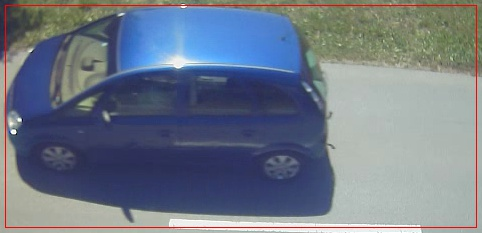
\includegraphics[width=0.49\textwidth]{Testversuche/GrabCut1.jpg}}
  \subfigure[Ergebnis des Algorithmus]{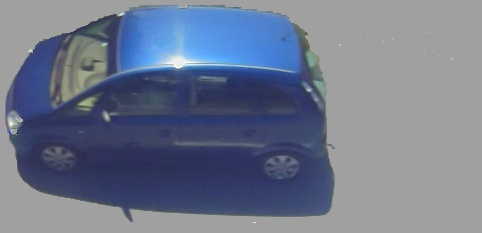
\includegraphics[width=0.49\textwidth]{Testversuche/GrabCut2.jpg}}
  \caption{Beispiel GrabCut}
  \label{bGrabCut}
\end{figure}

Auf dem linken Bild sind das Originalbild und der definierte Rahmen zu sehen, auf dem rechte Bild das Ergebnis dazu. Dem Ergebnis wurde ein grauer Hintergrund hinzugefügt, jedoch kann diese Farbe frei gewählt werden. Je nach Bild, welches verwendet wird, kann GrabCut schlechte bis hervorragende Resultate liefern. Dabei kommt es vor allem darauf an, wie starke Farbveränderungen im Hintergrund vorhanden sind. Bei diesem Algorithmus handelt es sich um eine komplexe Methode, welche selbst auf dem Computer einige Sekunden an Verarbeitungszeit benötigt. \cite{GrabCut}

\subsubsection{Schattenentfernung}
Als die ersten Testaufnahmen durchgeführt wurden, musste festgestellt werden, dass Schatten zu einem grossen Problem führen konnte. Dies trat vor allem dann auf, wenn die Sonne den Schatten des Verkehrsteilnehmers in richtung Kamera projezierte. Dadurch wurde der Bildausschnitt des Verkehrsteilnehmers grösser als er tatsächlich war, was weitere Auswertungen verfälschte. Aus diesem Grund wurde nach Möglichkeiten gesucht, um diesen Schatten zu entfernen, weshalb schlussendlich eine Funktion dafür geschrieben wurde.
Falls ein Schatten vorhanden war, konnte dies am Differenzbild erkannt werden. Dort traten jeweils, waagrecht betrachtet, zwei helle Streifen und dazwischen ein dunkler Abschnitt auf. Auffällig daran ist, dass die Breite der hellen Steifen fast gleich gross waren, was auf die Geschwindigkeit des Fahrzeugs zurückzuführen ist. Der helle Streifen entstand, wenn nur auf einem der beiden Bilder, welche für das Differenzbild zuständig waren, ein Schatten vorhanden war. Der dunkle Abschnitt zwischen den hellen Stellen entstand, wenn auf beiden Eingangsbildern bereits ein Schatten vorlag. Nachfolgende Abbildung (\fref{bBlurRemoveShadow}) zeigt die geschilderte Situation eines Differezbildes mit Schatten.

\begin{figure}[H]
  \centering
  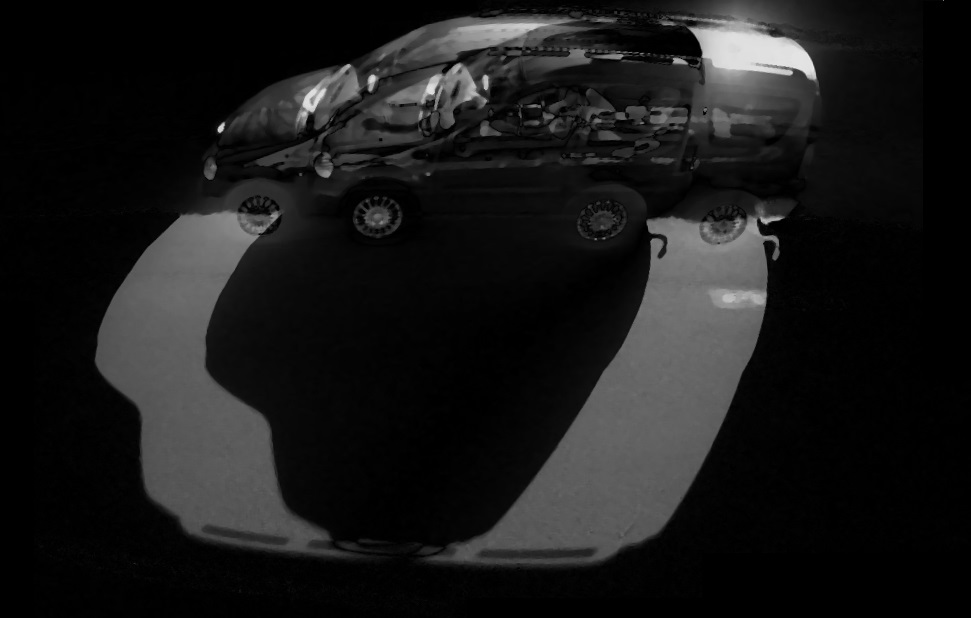
\includegraphics[height=0.3\textheight]{Testversuche/BlurRemoveShadow.jpg} 
  \caption{Differenzbild zur Demonstration des Schattens}
  \label{bBlurRemoveShadow}
\end{figure} 

Beim Algorithmus der Funktion wird jeweils 
\newpage
\section{Resultate}
\input{Resultate/EinzelnesGerät}
\subsection{System}
Ein System besteht aus mehreren Einzelgeräten, mit welchen, wie vorhin beschrieben, das Zählen, die Kategorisierung und die Geschwindigkeitsmessung durchgeführt werden. Es werden mehrere Geräte benötigt um den Verkehrsfluss in dem definiert begrenztem Gebiet darstellen zu können. Dabei werden die über den aufgenommenen Zeitstempel und die Fahrtrichtung der Verkehrsfluss statistisch rekonstruiert. Hierbei wird das vorhin erstellte Netzwerk des begrenzten Gebietes als Darstellungsgrundlage verwendet. Es werden zunächst die nächstgelegenen Geräte, welche auf direktem Weg erreichbar sind, identifiziert und von diesen die Daten des Feature Vektors extrahiert. Diese Daten werden dann nach dem Zeitstempel sortiert und mit einem Index versehen. Sind die Daten nun vorbereitet werden durch die Länge der Verbindungen und Geschwindigkeiten auf diesen, die voraussichtliche Durchfahrtszeit berechnet. Danach wird statistisch die höchste Wahrscheinlichkeit welchen Weg der Verkehrsteilnehmer nahm berechnet und eingezeichnet. Sind alle Geräte untereinander verglichen und alle Wege in dem Netzwerk eingezeichnet sind erhält man, wie unten dargestellt (\fref{bAuswertung}), eine Auswertung. 

\begin{figure}[H]
  \centering
  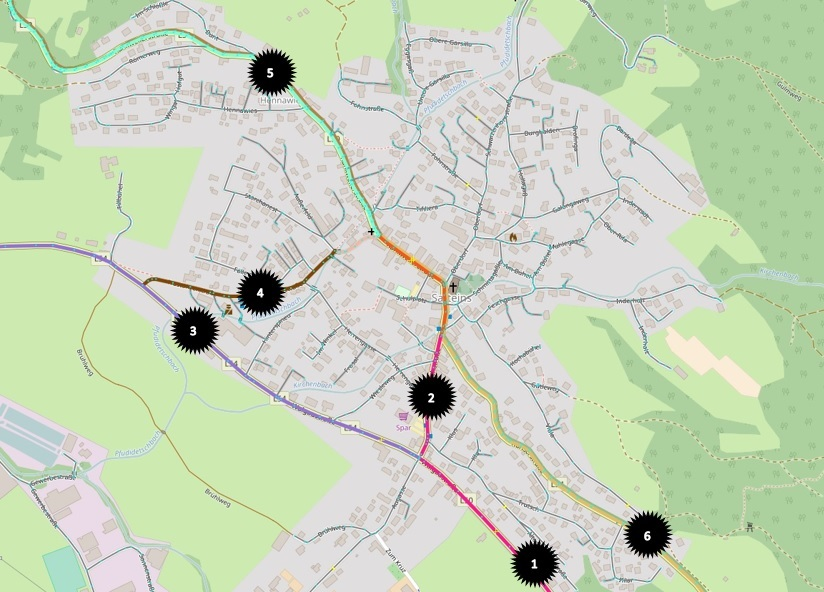
\includegraphics[width=0.6\textwidth]{Resultate/Auswertung.jpg} 
  \caption{Darstellung des Verkehrsflusses in Satteins.}
  \label{bAuswertung}
\end{figure}
In \tref{tVerkehrsfluss} ist der Verkehrsfluss von jedem Gerät zu seinem direkten Nachfolger tabellarisch dargestellt. 

\setlength\tabcolsep{5pt}

\begin{table}[H]
\centering
\begin{tabular}{|p{1.5cm}|p{1.5cm}|p{1.5cm}|p{1.5cm}|p{1.5cm}|p{1.5cm}|p{1.5cm}|p{1.5cm}|}
\hline
	von/nach & 1 & 2 & 3 & 4 & 5 & 6 & Out \\ \hline
	1 &  & 952 & 949 &  &  &  & 1703 \\ \hline
	2 & 326 & 0 & 279 & 105 & 434 & 275 & 0 \\ \hline
	3 & 996 & 0 &  &  &  &  & 1468 \\ \hline
	4 &  & 149 &  &  & 105 & 84 & 520 \\ \hline
	5 &  & 723 &  & 159 & 521 & 224 & 1668 \\ \hline
	6 &  & 313 &  & 78 & 426 &  & 327 \\ \hline
\end{tabular}
\caption{Tabelarische Darstellung des Verkehrsflusses.}
\label{tVerkehrsfluss}
\end{table}

\setlength\tabcolsep{0pt}
\subsection{Satteins}
Das Testgebiet des Systems war in Satteins. In den folgenden Punkten wird kurz das Gebiet beschrieben und wie die Daten erfasst wurden.
\subsubsection{Topologie}
Im nachfolgenen Bild (\fref{bSatteins}) ist die Topologie von Satteins dargestellt. In dieser Darstellung sind die Aufstellpunkte der sechs aufgestellten Geräte mit einem schwarzen Punkt schematisch markiert. Jedes dieser Geräte wurde an den Ein- und Ausfahrtspunkten, sowie an strategisch interessanten Verkehrspunkten platziert. Mit diesen sechs Geräten ist es möglich, den grössten Teil des Verkehrsflusses in Satteins quantitativ zu rekonstruieren. 

\begin{figure}[H]
  \centering
  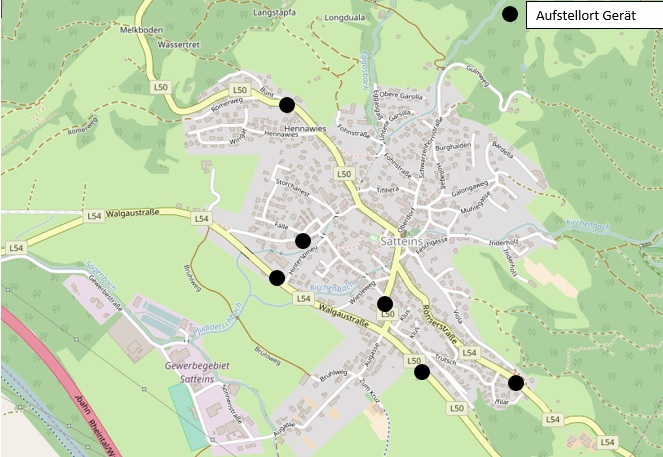
\includegraphics[width=0.99\textwidth]{Resultate/Satteins.jpg} 
  \caption{Topologie von Satteins. \cite{satteins}}
  \label{bSatteins}
\end{figure}

Mit Hilfe des Bildes (\fref{bGraph}) wird jede Abzweigung welche die Verkehrsteilnehmer nehmen können identifiziert und in der Berechnung des Verkehrsflusses beachtet. Dabei werden die Geräte schematisch auf einen Knotenpunkt, bei den Ein- und Ausfahrtsstrassen gelegt und die zwei Anderen werden auf die Mitte der Strasse projiziert. So lässt sich der Verkehrsfluss im Graphen darstellen und zu Letzt auf die Karte von Satteins zurück projizieren.

\begin{figure}[H]
  \centering
  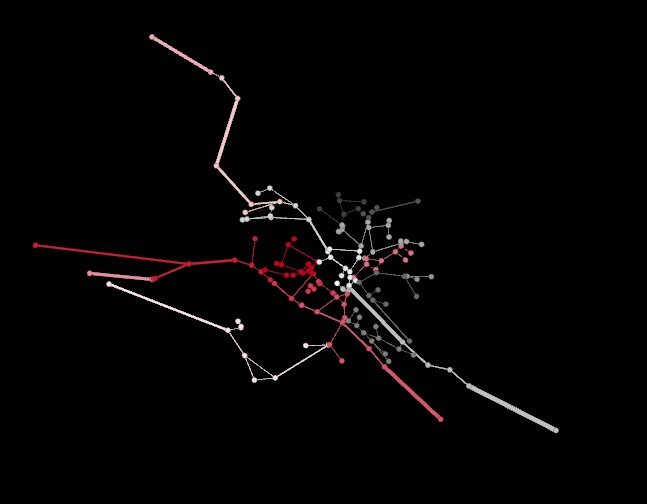
\includegraphics[width=0.99\textwidth]{Resultate/Topologie.jpg} 
  \caption{Graph des Verkehrsnetzes von Satteins.}
  \label{bGraph}
\end{figure}

\subsubsection{Erfassung der Daten}
Alle Daten welche die Geräte aufgezeichnet haben, wurden auf den internen SD-Karten abgespeichert und jeden zweiten Tag mittels Smartphone-Hotspot auf den Laptop übertragen. Dabei wurde bei jedem einzelnen Gerät der Feature Vektor, sowie der Temperaturverlauf heruntergeladen. Die Feature Vektoren der Geräte enthielten mehrere tausend Einträge mit vorbeifahrenden Verkehrsteilnehmern.
\newpage
\section{Ausblick}
\subsection{Features erweitern}
Je besser der Feature Vektor ist, desto einfacher und genauer kann die im Anschluss folgende Verkehrsverfolgung durchgeführt werden. Aus diesem Grund wäre es notwendig, aus den vorhandenen Bildern mehr Features zu erkennen. Nachfolgend sind deshalb einige Möglichkeiten aufgelistet, wie der Feature Vektor um zusätzliche Spalten erweitert werden könnte.

\subsubsection{Kategorisieren}
Ein mögliches Feature, das realisiert werden könnte, wäre beispielsweise das Kategorisieren der Verkehrsteilnehmer in mehrere Unterklassen. Mögliche Unterteilungen wären hierbei Fahrrad, Motorrad, PKW, Lieferwagen, Lastwagen, Traktor usw. Realisiert werden könnte dies über das Verhältnis der Länge und Breite und gleichzeitig der Anzahl an Pixeln der Blobs.

\subsubsection{Fahrzeuglänge \& -breite}
Ebenfalls plausibel könnte die Identifikation der Fahrzeuglänge oder -breite sein. Im besten Fall wäre diese direkt über das vorhandene Bild realisierbar. Dazu müsste aber ein Referenzmass für beide Fahrbahnen in Sichtweite der Kamera aufgetragen werden. Das Herauslesen von Längenmassen könnte jedoch auch über andere Sensoren realisiert werden.

\subsubsection{Farbe}
Die Farbe des Fahrzeugs wäre ein mögliches Merkmal, das unterschieden werden könnte. Damit dieses Feature gegenüber verschiedenen Belichtungen dennoch genügend resistent wäre, müsste dabei die erkannte Farbe in eine von etwa zehn Möglichkeiten eingeteilt werden. Ebenso müsste hier die Tageszeit beachtet werden, da eine Farbeerkennung unmöglich ist, wenn es draussen dunkel ist.

\subsubsection{Farbfläche}
Je grösser ein Auto ist, desto mehr Farbflächen sind vorhanden. Die Anzahl Pixel dieser Farbflächen könnte neben der Farbe ebenfalls dem Feature Vektor ergänzt werden. Damit eine Unterscheidung zwischen Fensterscheibe und Farbfläche durchgeführt werden kann, müsste vorgängig ein Clustering auf eine einheitliche Farbe durchgeführt werden.

\subsubsection{Sonderanbringungen}
Auf einigen Fahrzeugen befinden sich Sonderanbringungen wie Beschriftungen oder Bilder. Wenn diese Sonderanbringungen erkannt und bestenfalls abgespeichert werden könnten, so wäre dadurch eine eindeutige Wiedererkennung dieses Verkehrsteilnehmers realisierbar. Durchführbar wäre dies, wenn ein Algorithmus eine Sonderanbringung erkennt und davon ein zusätzliches Bild abspeichert.

\subsubsection{Nummerntafeln}
Mithilfe der Nummerntafeln wären die meisten Verkehrsteilnehmer ohne grossen Aufwand verfolgbar, da es nur wenig Fahrzeuge gibt die keine Nummerntafel besitzen. Problematisch wäre jedoch, dass die Ausrichtung der Kamera zum Erkennen der Kennzeichen an der falschen Position ist. Ebenso darf eine Nummerntafel aus rechtlichen Gründen nicht ohne weiteres aufgenommen werden, da damit ein Verkehrsteilnehmer eindeutig identifiziert werden kann.

\subsubsection{Geschwindigkeit}
Obwohl die Geschwindigkeit kaum für eine Verkehrsverfolgung genutzt werden kann, da sich diese während der Fahrt kontinuierlich ändern kann, so wäre diese Information für Gemeinden nützlich. Mit der Geschwindigkeit der Verkehrsteilnehmer könnte ein Durchschnitt ermittelt werden, der als Indikator dient, wie schnell tatsächlich am Gerät vorbeigefahren wurde.
\subsection{Vernetzung}
Im Moment funktioniert die Auswertung, indem die Daten vor Ort abgeholt und danach auf einem Rechner verarbeitet werden. Es wäre denkbar, dass die Geräte über ein Lora-WAN Netzwerk miteinander verbunden wären. Somit könnten die vorhandenen Feature Vektoren direkt übertragen werden, weshalb kein manuelles Abholen der Daten mehr nötig wäre. Das Monitoring der Geräte wäre so komplett online möglich. Die Temperaturen und Ausrichtung der Kamera könnten jederzeit überprüft werden. Lediglich eine Feinjustierung der Kamera und das Auswechseln des Akkus müsste vor Ort durchgeführt werden.
\subsection{Optimale Aufstellung}
Um eine optimale Verkehrsverfolgung durchführen zu können, müssen die Geräte an möglichst sinnvollen Stellen innerhalb der Ortschaft platziert werden. Diese Positionen könnten mithilfe eines Algorithmus berechnet werden. Somit könnte man die gewollte Ortschaft mithilfe eines Strassennetzes angeben und daraus würden die optimalen Standorte der Geräte ermittelt werden. Dafür wären zwei verschiedene Varianten denkbar. Zum einen, dass die Anzahl an Geräten angegeben werden kann, und daraus die Aufstellungen errechnet werden. Zum anderen, dass die Zahl der Geräte ebenfalls errechnet wird. Das Problem dabei wäre jedoch, dass selbst in kleineren Ortschaften riesige Mengen an Geräten benötigt würden.
\subsection{Echtzeitdarstellung}
Ausserdem ausführbar wäre eine Echtzeitdarstellung, womit ein Online-Monitoring realisierbar ist. Dabei wäre ein 24 Stunden Betrieb optimal. Jedoch ginge dies nur durch eine tiefere FPS-Zahl der Aufnahme, damit eine Nachtabschaltung nicht mehr notwendig wäre, um die Bilder fertig zu prozessieren. Die aufgenommenen Daten müssten direkt auf einen Server hochgeladen und auf einer Webseite bereitgestellt werden. Die Webseite könnte, in der gleichen Art wie "'Google Maps"', die verwendeten Geräte innerhalb der Ortschaft mit einigen zusätzlichen Informationen anzeigen. Plausible Informationen sind hierbei beispielsweise die Anzahl der Verkehrsteilnehmer, Anzahl der links- bzw. rechtsfahrenden Fahrzeuge, Geschwindigkeit des letzten Verkehrsteilnehmers oder die momentane Kerntemperatur des Gerätes. 

\input{Ausblick/ErweiterungDesGerätes}
\subsection{Spannungsversorgung}
Da sich die Batterien im Moment unterhalb der Strassenlaterne befinden, könnten Unbefugte in Berührung damit kommen oder diese gar entfernen. Aus diesem Grund wäre es sinnvoll, auf eine andere Art der Spannungsversorgung zu setzen. Damit die Akkumulatoren ebenfalls nicht ständig wieder aufgeladen werden müssen, wären Photovoltaik Zellen oder die gemeinsame Nutzung des Stroms der Strassenlaterne sinnvoll.
\newpage
\newpage
\section{Verzeichnisse}
\subsection{Abbildungsverzeichnis}
%\renewcommand\listfigurename{\vskip -1.5cm}
%\listoffigures
\subsection{Tabellenverzeichnis}
%\renewcommand\listtablename{\vskip -1.5cm}
%\listoftables
\subsection{Literatur}
%\renewcommand\refname{\vskip -1cm}
%\bibliography{../99_Literaturverzeichnis/LiteraturKopie}
\input{EidestattlicheErklärung}
\section{Anhang}

- Verwendetes Ubuntu Image (USB Stick)
\newpage
\end{document}